\section{Introduction} Canonical correlation analysis (CCA) is a classical joint
multidimensional dimensionality reduction algorithm for inferring or learning latent
correlations present in two datasets \cite{hotelling1936relations}. CCA learns a linear
transformation for each dataset such that the transformed features have maximal
correlation. Often, canonical correlation analysis is the first step in algorithms that
aim to fuse the information in the datasets to improve inference in the context of tasks
involving the detection, estimation, classification, and prediction of correlated
signals. CCA has been used in in machine learning \cite{hardoon2004canonical,
  dhillon2011multi, zhai2015instance, hardoon2006correlation,chaudhuri2009multi}, medical
signal processing, \cite{ correa2010canonical,arbabshirani2010comparison,
  khalid2013improving, lin2013identifying, seoane2014canonical, zhang2013l1,
  nakanishi2014enhancing, spuler2014spatial, kuzilek2014comparison},
economics \cite{todros2012measure}, climatology \cite{wilks2014probabilistic,
  prera2014using, steward2014assimilating}, and classical signal processing like Wiener
filters \cite{scharf1998wiener} and array processing \cite{ge2009does}.

In practice, when the population covariance and cross-covariance matrices of the two
datasets are unknown, they must be estimated from data. Empirical CCA relies on plug-in
estimates for these quantities. When the number of samples is large relative to the
combined dimensionality of the two datasets, empirical CCA performs well in the sense that
the empirical canonical correlation coefficients can be used to reliably infer the
presence of correlated signals buried in noise. However, when the sample size is less than
the combined dimensionality of the datasets the nthe empirical canonical correlation
coefficients will deterministically equal one, \textit{irrespective of whether there is a
  correlated signal in the datasets} \cite{pezeshki2004empirical}. This observation
led Pezeshki, Scharf et al to correctly conclude that in this regime
\begin{quote}
    ... the empirical canonical correlations are defective and may not be used as  estimates of canonical correlations between random
    variables.
\end{quote}
He et al. \cite{ge2009does} used extensive simulations to make a similar observation about
the deficiencies of empirical CCA in the sample size limited regime.

Recently, Bao et al \cite{bao2014canonical} rigorously studied the limiting behavior of
the empirical canonical correlation coefficients for the setting where the population
covariance matrix is arbitrary but the cross-covariance matrix is low rank. Their work
establishes the fundamental asymptotic limits of empirical CCA based detection of
correlated signals in noise in the general setting where the dimensionality of the system
is of the same order as the number of samples used to form the empirical covariance and
cross-covariance matrices. A conclusion from this analysis is the existence of a phase
transition threshold, which separates the regime where the low-rank signals are correlated
and can be detected using empirical CCA from a regime where they remain correlated but
cannot be detected using empirical CCA. More importantly, this phase transition threshold
depends explicitly on the degree of correlation between the signals. Particularly, as the
correlation decreases, the minimum (eigen) signal-to-noise ratio (SNR) above which
reliable detection is possible increases. Moreover, when there are not enough samples
relative to the combined dimensionality of the system, which includes the regime studied
by Pezeshki et al \cite{pezeshki2004empirical}, then the empirical correlation
coefficients will tend to one regardless of whether there is a correlated signal or not,
thereby crippling the inferential utility of empirical CCA based detection for the kinds
of high-dimensional ``large-$p$-relatively-small-$n$'' type problems that arise in modern
signal processing and machine learning
\cite{johnstone2008multivariate,fujikoshi2009high,wainwright2009sharp,yang2015computational,janson2015eigenprism}.

These results might convey to a practitioner that it is not theoretically possible to
detect the presence of correlated signals in two datasets for modern and emerging high
dimensional inferential problems. It is against this backdrop that we revisit this problem
from first principles. We consider the setting where the individual matrix-valued datasets
can be modeled as low-rank-correlated-signals-plus-noise type matrices; this model is
motivated by the ubiquity and success of low-rank models in practice
\cite{eckart1936approximation,candes2011robust,belkin2003laplacian,bach2003kernel,candes2011tight}. We
utilize the results of Bao et al \cite{bao2014canonical} and Pezeshki et al
\cite{pezeshki2004empirical} to establish the fundamental limits of empirical CCA for this
model. We then reconsider the connection between the canonical correlation coefficients
and angles between subspaces, and propose a simple modification to empirical CCA, which
builds on the work in \cite{nadakuditi2011fundamental}, that we label Informative CCA
(ICCA). We show that empirical CCA infers the presence of latent correlations by
considering the singular values of a matrix formed using all of the right singular vectors
of the individual signal-plus-noise matrices. In the regime where empirical CCA fails, a
subset of the right singular vectors of the individual matrices are ``informative'', i.e.,
positively correlated with the latent signal singular vectors. This insight motivates our
development of ICCA which infers the presence of latent correlations by considering the
singular values of a matrix formed using only these ``informative'' principal right
singular vectors of the individual signal-plus-noise matrices. In the setting where the
noise matrix is i.i.d. Gaussian, we also provide a principled approach, that leverages
using results from random matrix theory \cite{nadakuditi2010fundamental}, for selecting
the number of informative components.

We then establish the fundamental limits of inference using ICCA and bring into sharp
focus phase transitions that separate a regime where ICCA reliably infers (in an
asymptotic sense that we make precise) the presence of a correlated signal from a regime
where the correlation is present but ICCA fails. By comparing the derived fundamental
limits of ICCA with the fundamental limits for empirical CCA derived by Bao et al
\cite{bao2014canonical}, we are able to show that ICCA provably succeeds in reliably
detecting correlations in the sample deficient regime where empirical CCA provably
fails. Throughout this paper, when we say an algorithm ``provably succeeds'' we will mean
that the difference between the test statistic for the pure noise setting versus
correlated signal setting is almost surely positive. When we say that that the algorithm
``provably fails'' we mean that this difference is almost surely zero. The analysis also
reveals that the detection performance of ICCA does not depend on the correlation
coefficient, a very nice benefit over empirical CCA whose performance does depend on the
correlation coefficient. We show that our algorithm extends readily to the widely
considered missing data setting
\cite{candes2006stable,candes2009exact,cai2010singular,candes2010matrix,candes2010power}
and our analysis reveals that the benefits of ICCA over empircal CCA hold for this setting
as well as for a class of generalized noise models such as those considered in
\cite{benaych2012singular}.

The ICCA algorithm itself is relatively straightforward and we suspect that many
practitioners have used it or are already using it because they have observed numerically
that it ``works'' when empirical CCA does not. The main contribution of this work is the
establishment of a principled, mathematically rigorous framework that justifies the use of
ICCA based detection of correlated signals and the development of rigorous performance
guarantees for when we expect ICCA to succeed and the sorts of performance improvements we
can expect relative to empirical CCA. To the best of our knowledge, this is novel; in a
subsequent paper we will provide performance guarantees for canonical vectors estimated
using ICCA. The analysis of ICCA uses results established in
\cite{benaych2012singular,benaych2011eigenvalues} and extends them to consider the new
test statistic proposed herein. To that end, Theorem \ref{th:v_ip}, which is a crucial
tool used to prove Theorem \ref{th:khat_lims}, might be of independent interest to readers
with theoretical leanings. In addition to our many main results, we present some
theoretical conjectures that we believe to be true but which we were not able to
prove. Proving these conjectures will require a precise characterization of the limiting
behavior of of the empirical canonical correlation coefficients and their fluctuations and
the fluctuation behavior of the ICCA test statistic. We provide empirical evidence to lend
credence to our conjectures and hope that this will provide theoretically inclined readers
with an impetus for bridging this gap.

This paper is organized as follows. We provide the linear
low-rank-correlated-signal-plus-noise data model in Section \ref{sec:chpt4:model}. We then
derive the solution of CCA in Section \ref{sec:chpt4:cca} and show how to estimate the
number of correlated components from its solution. In Section \ref{sec:chpt4:emp_cca}, we
derive the empirical version of CCA using sample covariance matrices, highlight the
connection to angles between subspaces, and exploit that connection to present our
proposed ICCA algorithm. We then provide statistical tests to estimate the number of
correlated components present in the datasets for both empirical CCA and ICCA. We
summarize our main theoretical results in Section \ref{sec:chpt4:cca_theory}, highlighting
fundamental detection limits for empirical CCA (based on the work of Bao et al
\cite{bao2014canonical}) and ICCA (based on results we derive in this paper). We extend
this analysis to the missing data and non-Gaussian noise settings.  We verify these
theoretical results both on simulated data and real-world datasets in Section
\ref{sec:chpt4:emp}. Finally, we provide concluding remarks in Section
\ref{sec:chpt4:concl}.


\section{Setup}\label{sec:chpt4:model}

We assume that we are given $n$ observations of each dataset, which we stack columnwise to
form two data matrices
\begin{subequations}\label{eq:chpt4:data}
\beq
 X = [x_1,\dots,x_n]
\eeq
\beq
 Y = [y_1,\dots,y_n].
\eeq
\end{subequations}
It is important to note that the number of observations of each dataset must be the same and
that the observations come in pairs. For $i=1,\dots,n$, let $\xii\in\complex^{p\times 1}$
and $\yii\in\complex^{q\times 1}$ be modeled as
\begin{subequations}\label{eq:chpt4:data_model}
\beq
\xii = \Ux\sx + \zx
\eeq
\beq
\yii = \Uy\sy + \zy,
\eeq
\end{subequations}
where $\Ux^H\Ux=I_{\kx}$, $\Uy^H\Uy=I_{\ky}$, $\zx\simiid\mathcal{CN}(0,I_p)$ and
$\zy\simiid\mathcal{CN}(0,I_q)$. Furthermore, assume that
\be\ba
&\sx\sim\mathcal{CN}(0,\Tx)\\
&\sy\sim\mathcal{CN}(0,\Ty),\\
\ea\ee
where
\begin{subequations}\label{eq:chpt4:thetas}
\beq
\Tx=\diag\left(\left(\tx_1\right)^2,\dots,\left(\tx_{\kx}\right)^2\right)
\eeq
\beq
\Ty=\diag\left(\left(\ty_{1}\right)^2,\dots,\left(\ty_{\ky}\right)^2\right).
\eeq
\end{subequations}
Assume that $\zx$ and $\zy$ are
mutually independent and independent from both $\sx$ and $\sy$. Finally, assume that
\be
\E{\sx \sy^H} \defeq \Kxy = \Tx^{1/2}\Pxy\Ty^{1/2},
\ee
where the entries of $\Pxy$ are $-1\leq |\rho_{kj}| \leq 1$ and represent the correlation
between $\sx^{(k)}$ and $\sy^{(j)}$. For reasons to be made clear later, define
\be
\Kxytil = \left(\Tx+I_{\kx}\right)^{-1/2}\Kxy\left(\Ty+I_{\ky}\right)^{-1/2}
\ee
and define the singular values of $\Kxytil$ as
$\kappa_1,\dots,\kappa_{\min(\kx,\ky)}$. Under this model, we define the following
covariance matrices
\begin{subequations}\label{eq:chpt4:true_scm}
\beq\label{eq:chpt4:rxx}
\E{\xii\xii^H} = \Ux\Tx\Ux^H + I_p \defeq \Rxx
\eeq
\beq\label{eq:chpt4:ryy}
\E{\yii\yii^H} = \Uy\Ty\Uy^H + I_q \defeq \Ryy
\eeq
\beq\label{eq:chpt4:rxy}
\E{\xii\yii^H} = \Ux\Kxy\Uy^H \defeq \Rxy.
\eeq
\end{subequations}
Note that we may write $\sx=\Tx^{1/2} v_{x,i}$ and $\sy=\Ty^{1/2} v_{y,i}$ where
$v_{x,i}\sim\mathcal{CN}(0,I_{k_x})$ and $v_{y,i}\sim\mathcal{CN}(0,I_{k_y})$ are
independent random vectors. Defining $\Zx = [z_{x,1},\dots,z_{x,n}]$, $\Zy =
[z_{y,1},\dots,z_{y,n}]$, $\Vx=[v_{x,1},\dots,v_{x,n}]$, and $\Vy=[v_{y,1},\dots,v_{y,n}]$, we may write our data
matrices in (\ref{eq:chpt4:data}) as the sum of a low-rank signal matrix and noise
matrix
\begin{subequations}\label{eq:chpt4:data_matrices}
\beq
 X = \Ux\Tx^{1/2}\Vx^H + \Zx
\eeq
\beq
 Y = \Uy\Ty^{1/2}\Vy^H + \Zy.
\eeq
\end{subequations}

\section{Canonical Correlation Analysis and its variants}\label{sec:chpt4:cca}

Canonical Correlation Analysis (CCA) is a dimensionality reduction algorithm that finds
linear transformations for $\xii$ and $\yii$ such that in the projected spaces, the
transformed variables
are maximally correlated. Specifically, CCA solves the following optimization problem
\beq\label{eq:chpt4:opt_cca}
\rhocca =\max_{\wx,\wy} \frac{\wx^H\Rxy\wy}{\sqrt{\wx^H\Rxx\wx}\sqrt{\wy^H\Ryy\wy}},
\eeq
where $\wx$ and $\wy$ are called canonical vectors and $\rhocca$ is called the canonical
correlation coefficient. Notice that we can scale $\wx$ and
$\wy$ and still achieve the same objective function. Therefore, we may constrain the
canonical variates to have unit norm, resulting in the optimization problem
\beq\label{eq:chpt4:cca}\ba
&\max_{\wx,\wy} &&\wx^H\Rxy\wy\\
&\text{subject to} && \wx^H\Rxx\wx = 1\\
&&& \wy^H\Ryy\wy=1.\\
\ea\eeq
Substituting the change of variables $\wxt=\Rxx^{1/2}\wx$ and
$\wyt=\Ryy^{1/2}\wy$ in (\ref{eq:chpt4:cca}) results in the following optimization problem
\beq\label{eq:chpt4:cca_svd}\ba
&\max_{\wxt,\wyt} &&\wxt^H\Rxx^{-1/2}\Rxy\Ryy^{-1/2}\wyt\\
&\text{subject to} && \wxt^H\wxt = 1\\
&&& \wyt^H\wyt=1.\\
\ea\eeq
Examining the optimization problem in (\ref{eq:chpt4:cca_svd}), we can immediately see that the
solution to CCA may be solved via the SVD of the matrix
\beq\label{eq:chpt4:c_cca}
\Ccca = \Rxx^{-1/2}\Rxy\Ryy^{-1/2}.
\eeq
Define $\Ccca=FKG^T$ as the SVD of $\Ccca$ where $F$ is an unitary
$p\times p$ matrix with columns $f_1,\dots,f_p$, $G$ is a unitary $q\times q$ matrix with
columns $g_1,\dots,g_q$, and
$K=\diag(k_1,\dots,k_{\min(p,q)})$ is a $p\times q$ matrix whose diagonal elements are the
singular values of $\Ccca$. Therefore, the solution to (\ref{eq:chpt4:cca_svd}) is
\be\ba
\wxt = f_1\\
\wyt = g_1\\
\rho_{\text{cca}} = k_1.\\
\ea\ee
We can obtain higher order canonical correlations and vectors by taking successive singular
value and vector pairs. From this solution, it is clear that the number of non-zero
canonical correlation coefficients is exactly equal to the rank of $\Ccca$. Recalling the
definitions in (\ref{eq:chpt4:true_scm}),
$\Rxx$ and $\Ryy$ are non-singular so we have that
\be\ba
&\text{\# canonical correlation}&&=\rank(\Ccca)\\
&\text{   coefficients}&& = \rank(\Rxx^{-1/2}\Rxy\Ryy^{-1/2})\\
&&& = \rank(\Rxy)\\
&&& = \rank(\Kxy)\\
&&&\defeq k.\\
\ea\ee
Therefore, when we know all parameters, $k$ is exactly the number of non-zero singular
values of $\Kxy$. We note that $k\leq\min(\kx,\ky)$. Our  objective is to infer the number of non-zero canonical correlation coefficients from data.

\section{Detection of correlated signals using empirical and informative CCA}\label{sec:chpt4:emp_cca}
In many applications, we do not know the covariance matrices $\Rxx$, $\Ryy$, and $\Rxy$
\textit{a priori} and hence the quantities in
(\ref{eq:chpt4:true_scm}) are unknown. Consequently, we cannot determine the number
of canonical correlation coefficients by examining the rank of $\Rxy$. Instead, given
the data matrices in (\ref{eq:chpt4:data}), we form estimates of our unknown covariance
matrices via
\be\ba
& \Rxxhat = \frac{1}{n}XX^H\\
& \Ryyhat = \frac{1}{n}YY^H\\
& \Rxyhat = \frac{1}{n}XY^H.\\
\ea\ee
Define the data SVDs of the matrices in (\ref{eq:chpt4:data}) as
\be\ba
& X = \Uxhat\Sigxhat\Vyhat^H\\
& Y = \Uyhat\Sigyhat\Vyhat^H\\
\ea\ee
and trimmed matrices
\begin{subequations}\label{eq:chpt4:cca_trimmed}
\beq
 \Uxtil = \Uxhat\left(:,1:\min(p,n)\right)
\eeq
\beq
 \Vxtil = \Vxhat\left(:,1:\min(p,n)\right)
\eeq
\beq
 \Uytil = \Uyhat\left(:,1:\min(q,n)\right)
\eeq
\beq
 \Vytil = \Vyhat\left(:,1:\min(q,n)\right).
\eeq
\end{subequations}
Substituting the SVDs of sample analogs of the matrices in (\ref{eq:chpt4:c_cca}), reveals the insight (\cite[Eq. (6)]{nadakuditi2011fundamental}) that the matrix $\Ccca$ can be estimated as
\beq\label{eq:chpt4:cccahat}
\Cccahat = \Uxtil\Vxtil^H\Vytil\Uytil^H.
\eeq
We denote the singular values of this matrix by $\rhohatcca^{(j)}$ for $j=1,\dots,\min(p,q)$; these are precisely the empirical CCA correlation coefficients. Empirical CCA can return up
to $\min(p,q)$ canonical correlations; however, we know from the data model in
(\ref{eq:chpt4:data_model}) that $X$ and $Y$ have $\kx$ and $\ky$ underlying signals,
respectively. As $\kx$ and $\ky$ are unknown, let $\kxhat$ and $\kyhat$ be estimates of
the number of underlying signals in each dataset. As a consequence of (\ref{eq:chpt4:opt_cca})
we define the
plug-in estimates of $\rhocca$, as the $\min(\kxhat,\kyhat)$ singular values of $\Cccahat$ as
\beq\label{eq:chpt4:rhohatcca}
\rhohatcca^{(1)},\dots,\rhohatcca^{(\min(\kxhat,\kyhat))}.
\eeq
For now, we assume that we are given $\kxhat$ and $\kyhat$, but we will return to the
problem of estimating these parameters from data. To estimate the canonical vectors, we
use the corresponding left and right singular vectors of $\Cccahat$, $f_i$ and $g_i$ to
form
\begin{subequations}\label{eq:chpt4:cca_vects}
\beq
 w_x^{(i)} = \Rxxhat^{-1/2}f_i
\eeq
\beq
 w_y^{(i)} = \Ryyhat^{-1/2}g_i.
\eeq
\end{subequations}

When the number of samples is less than the combined dimension of the datasets ($n<p+q$),
the largest singular value of $\Cccahat$ is deterministically one
\cite{pezeshki2004empirical}, regardless of whether an underlying correlation actually
exists between the datasets. This is a very unfortunate property of empirical CCA as many of the motivating
applications operate in this low-sample, high-dimensionality regime. A key observation in
\cite{nadakuditi2011fundamental} shows that the singular values of $\Cccahat$ are exactly
the same as the singular values of $\Vxtil^H\Vytil$. This is a $\min(p,n)\times\min(q,n)$
matrix that uses all right singular vectors of each dataset corresponding to a non-zero
singular value. However, under the low-rank signal-plus-noise model,
\cite{nadakuditi2011fundamental} shows that only a few of the right singular vectors
actually contain \textit{informative} signal. Therefore, by trimming $\Vxtil$ and $\Vytil$
to have only $\kxhat$ and $\kyhat$ columns, we can avoid the performance loss of empirical
CCA in the sample deficient regime. Define the trimmed data SVDs
\begin{subequations}\label{eq:chpt4:trimmed_svds}
\beq
 \Uxcir = \Uxhat\left(:,1:\kxhat\right)
\eeq
\beq
 \Vxcir = \Vxhat\left(:,1:\kxhat\right)
\eeq
\beq
 \Uycir = \Uyhat\left(:,1:\kyhat\right)
\eeq
\beq
 \Vycir = \Vyhat\left(:,1:\kyhat\right).
\eeq
\end{subequations}
Given these definitions, we define the informative CCA (ICCA) matrix
\beq\label{eq:chpt4:ciccahat}
\Ciccahat = \Uxcir\Vxcir^H\Vycir\Uycir^H.
\eeq
Similar to empirical CCA, define the top $\min(\kxhat,\kyhat)$ singular values of $\Ciccahat$ as
\beq\label{eq:chpt4:rhohaticca}
\rhohaticca^{(1)},\dots,\rhohaticca^{(\min(\kxhat,\kyhat))}.
\eeq
To estimate the ICCA canonical vectors, we
use the corresponding left and right singular vectors of $\Ciccahat$, $f_i$ and $g_i$, to
form
\begin{subequations}\label{eq:chpt4:icca_vects}
\beq
 w_x^{(i)} = \Rxxhat^{-1/2}f_i
\eeq
\beq
 w_y^{(i)} = \Ryyhat^{-1/2}g_i.
\eeq
\end{subequations}
For completeness, we will address the problem of estimating the canonical vectors in a
subsequent paper.

\subsection{New Statistical Tests for Correlation Detection}\label{sec:chpt4:new_test}
 Given the canonical correlation estimates from CCA and ICCA, we can
estimate the number of canonical correlations using the test statistics
\begin{subequations}\label{eq:chpt4:khats}
\beq
 \khatcca = \sum_{i=1}^{\min(p,q)} \indicator_{\left\{\left(\rhohatcca^{(i)}\right)^2
     >\taucca\right\}}
\eeq
\beq
 \khaticca = \sum_{i=1}^{\min(\kxhat,\kyhat)}
 \indicator_{\left\{\left(\rhohaticca^{(i)}\right)^2 >\tauicca\right\}},
\eeq
\end{subequations}
where $\indicator_{\left\{\cdot\right\}}$ is the indicator function and
\begin{subequations}\label{eq:chpt4:taus}
\beq
 \taucca = F^{-1}_{\text{cca}}(1-\alpha)
\eeq
\beq
 \tauicca = F^{-1}_{\text{icca}}(1-\alpha).
\eeq
\end{subequations}
Here $F_{\text{cca}}$ and $F_{\text{icca}}$ are the distributions of the square of the largest singular
value of $\Cccahat$ and $\Ciccahat$ for the null setting where $\Vxtil$ and $\Vytil$ are the
$\min(n,p)$ and $\min(n,q)$ columns of two independent Haar (or isotropically random)
distributed $n\times n$ matrices. The exact distribution of the squared singular values of
$\Cccahat$ and $\Ciccahat$ in
the null model is given in \cite{constantine1976asymptotic}. The distributions of the
square of the largest singular value of $\Cccahat$ and $\Ciccahat$ in the null model may be
approximated to second-order by the Tracy-Widom law \cite{johnstone2008multivariate} as
\begin{subequations}\label{eq:chpt4:taus}
\beq
\taucca \approx \sigma_{p,q,n}\twrc^{-1}(1-\alpha) + \mu_{p,q,n},
\eeq
\beq
\tauicca \approx \sigma_{kxhat,\kyhat,n}\twrc^{-1}(1-\alpha) + \mu_{\kxhat,\kyhat,n},
\eeq
\end{subequations}
where $\sigma_{n,p,q}$ is a scaling parameter and $\mu_{n,p,q}$ is a centering
parameter and $\twrc$ is the appropriate Tracy-Widom law for either real or complex
data. See Tables III and IV of \cite{nadakuditi2010fundamental} for values of these
parameters as well as algorithms to determine $\kxhat$ and $\kyhat$. For a similar
high dimensional analysis, see \cite{fujikoshi2009high}.

\begin{comment}
We note that
$\sigma=o(n^{-1/3})$ and $\mu=o(n^{-1/2})$ so that as $n\to\infty$ (for fixed $p$, $q$,
$\kxhat$, and $\kyhat$), $\taucca$ and $\tauicca$ both tend towards zero.

\subsection{Classical Wilks Lambda Correlation Test}\label{sec:chpt4:wilks}
To test the significance of the empirical CCA canonical correlation estimates, classical
methods \cite{hardle2007applied,bartlett1954note} employ the Wilks likelihood ratio statistic,
\be
\Lambda\left(\rhohatcca^{(1)},\dots,\rhohatcca^{(\min(p,q))}\right) = -\left(n-\frac{p+q
    +3}{2}\right)\log\left(\prod_{i=1}^k\left(1-\rhohatcca^{(i)2}\right)\right),
\ee
which approximately follows a chi-square distribution
\be
\Lambda\left(\rhohatcca^{(1)},\dots,\rhohatcca^{(\min(p,q))}\right)\sim\chi_{pq}^2.
\ee
To determine significance of $\rhohatcca^{(1}$, we
compare the statistic against a threshold to achieve a desired false alarm rate via
\beq\label{eq:chpt4:wilks}
\Lambda\left(\rhohatcca^{(1)},\dots,\rhohatcca^{(\min(p,q))}\right) \siggtrless \eta,
\eeq
where $\eta = Q^{-1}_{\chi_{pq}^2}\left(1-\alpha\right)$, $\alpha$ is a desired
probability of false alarm and $Q$ is the inverse cumulative distribution function of the
chi squared distribution with $p\times q$ degrees of freedom.

From our derivation in Section \ref{sec:chpt4:new_test}, we observe that the classical
Wilk's Lambda test is suboptimal for testing the presence of a correlation in the low-rank
signal-plus-noise model for both empirical CCA and ICCA. The Tracy-Widom distribution is
the exact distribution of the singular values of $\Cccahat$ and $\Ciccahat$ in the
asymptotic setting. Therefore, using the Wilk's test statistic to test the significance of
empirical CCA and ICCA singular values will either result in a decrease in detection
ability or increase if false alarm rate compared to the Tracy-Widom based tests.

\end{comment}
\section{Main Results}\label{sec:chpt4:cca_theory}

In this section we summarize the main theoretical results for empirical CCA and our new
ICCA algorithm. We derive parameter regimes where the estimates in (\ref{eq:chpt4:khats})
correctly infer the presence of correlated signals. We then extend these
results to include the cases when the data matrices have missing entries and when the
additive noise of the data model in (\ref{eq:chpt4:data_model}) is not Gaussian.

\subsection{Empirical CCA}\label{sec:empircal CCA limits}

\begin{prop}\label{prop:pezeshki}
Let $n,p,q\to\infty$ such that $p/n\to c_x$ and $q/n\to c_y$. Let $p+q\leq n$. Then the
largest singular value of $\Cccahat$ generated from data modeled in (\ref{eq:chpt4:data_model})
behaves as
\be
\rhohatcca^{(1)} = 1.
\ee
\end{prop}
\begin{proof}
See \cite{pezeshki2004empirical}, page 996.
\end{proof}

A consequence of Proposition \ref{prop:pezeshki} is that the sample canonical correlation
coefficients obtained using empirical CCA will equal one even when there is no correlation
signal present in the datasets. We now establish the limiting behavior of the sample
canonical correlation coefficients for the regime where they are not deterministically
equal to one. The following proposition is a result presented in \cite{bao2014canonical},
adopted using our notation.

\begin{prop}\label{prop:bao}
Let $n,p,q\to\infty$ such that $p/n\to c_x$ and $q/n\to c_y$. Assume that $p+q<n$. For
$i=1,\dots,\min(\kx,\ky)$, let $\rhohatcca^{(i)}$ be the $i$-th largest singular value
of $\Cccahat$ generated from data modeled in (\ref{eq:chpt4:data_model}). Then these singular
values behave as
{\footnotesize \beq\label{eq:chpt4:bao_cca}
\rhohatcca^{(i)} \convas \begin{cases} \sqrt{\kappa_i^2\left(1-c_x+\frac{c_x}{\kappa_i^2}\right)\left(1-c_y+\frac{c_y}{\kappa_i^2}\right)} & \textrm{ if }  \kappa_i^2 \geq r_c \\ \sqrt{d_r} & \textrm{ if } \kappa_i^2<r_c\end{cases}
\eeq}
where $\kappa_i$ are the singular values of $\Kxytil$ and
\beq\label{eq:chpt4:rc}
 r_c = \frac{c_xc_y+\sqrt{c_yc_y(1-c_x)(1-c_y)}}{(1-c_x)(1-c_y) +
  \sqrt{c_xc_y(1-c_x)(1-c_y)}}
\eeq
and
\beq\label{eq:chpt4:dr}
 d_r = c_x+c_y-2c_xc_y+2\sqrt{c_xc_y(1-c_x)(1-c_y)}.
\eeq
\end{prop}
\begin{proof}
  See \cite{bao2014canonical} for original proof our see our appendix for a proof
  providing the necessary mathematical manipulations to transform our data model to the
  one used in \cite{bao2014canonical}.
\end{proof}

Proposition \ref{prop:bao} brings into sharp focus the existence of a phase transition
that separates a regime where the sample canonical correlation coefficients can be used to
infer the presence of a correlated signal from a regime where it cannot. The phase
transition boundary depends on the correlation between the signals in the two datasets via
the $\kappa_i$ quantity. We will empirically verify this result by \cite{bao2014canonical}
and use it as a baseline for CCA to which we will compare our new estimate, ICCA.

The empirical CCA estimate of the number of correlated components is given by  (\ref{eq:chpt4:khats}). Since $\taucca \to \sqrt{d_r}$, we expect (\ref{eq:chpt4:khats}) to return the number of singular values greater than $\sqrt{d_r}$. Let
\beq\label{eq:chpt4:keff_cca}
k_{\text{eff}}^{\text{cca}} =  \sum_{i=1}^k\indicator_{\{\kappa_i^2 > r_c\}},
\eeq
denote the effective number of correlated components detectable by empirical CCA. Note
that, by definition, $k_{\text{eff}}^{\text{cca}} \leq k$. Proposition \ref{prop:bao}
shows that $k_{\text{eff}}^{\text{cca}}< k$ whenever some of the singular values are below
the phase transition threshold $r_c$. These observations lead to the following conjecture.

\begin{conj}\label{conj:khat_lims}
In the same setting as Proposition \ref{prop:bao}, we have that
\be\ba
& \Prob{\khatcca = k_{\text{eff}}^{\text{cca}}}\to 1 &&\text{ if } \kappa_k^2 >r_c \text{ and } n>p+q\\
\ea\ee
where $\kappa_i$ are the singular value of $\Kxytil$ and $r_c$ is given in
(\ref{eq:chpt4:rc}).
\end{conj}

\begin{comment}
\begin{proof}
  The conditions for the consistency of the CCA estimate follows from
  (\ref{eq:chpt4:bao_cca}). From this equation, we observe that the square of the smallest
  non-zero singular value of $\Kxytil$, $\kappa_k$, must be larger than the constant $r_c$
  for the canonical correlation estimate to be different statistically from noise.
\end{proof}
\end{comment}

\subsection{ICCA}\label{sec:chpt4:new_results}

We now provide analogous performance guarantees for ICCA and establish conditions that can
be used to identify broad regimes where ICCA reliably detects correlations but empirical
CCA, based on Proposition \ref{prop:bao}, does not.  Our analysis of ICCA relies on the
characterization of the entries of the matrix $\Vxcir^H\Vycir$. To that end, we provide the
following intermediate theorem.

\begin{Th}\label{th:v_ip}
Let $\Vxcir$ and $\Vycir$ be the trimmed right singular vectors defined in
(\ref{eq:chpt4:trimmed_svds}) of the data matrices generated from the data model in
(\ref{eq:chpt4:data_model}). In the asymptotic setting of Theorem \ref{th:w_ip} with
$p/n\to c_x$ and $q/n\to c_y$
\be
\left|\left[\Vxcir^H\Vycir\right]_{ij}\right|\convas \left|\kxy_{ij}\right|\alpha_{x,i}\alpha_{y,j},
\ee
where
\begin{subequations}\label{eq:chpt4:alphas}
\beq\label{eq:chpt4:alpha_x}
\alpha_{x,i} = \sqrt{1 - \frac{c_x + \tx_i}{\tx_i(\tx_i + c_x)}} \qquad \textrm{ if }
  \tx_i > c_x^{1/4},
\eeq
and
\beq\label{eq:chpt4:alpha_y}
\alpha_{y,j} = \sqrt{1 - \frac{c_y + \ty_j}{\ty_j(\ty_j + c_x)}} \qquad \textrm{ if }
  \ty_j > c_y^{1/4},
\eeq
\end{subequations}
and $ \kxy_{ij}$ are the entries of $\Kxy$.
\end{Th}
\begin{proof}
See Appendix for proof and Theorem \ref{th:w_ip}.
\end{proof}


\begin{comment}
A consequence of Theorem \ref{th:v_ip} is that when $\kxhat=\kx$ and $\kyhat=\ky$, the
smallest singular value of $\Vxcir^H\Vycir$ is greater than zero. Armed with this insight,
we are now in position to prove the consistency of the ICCA estimates of the number of
correlated signals in (\ref{eq:chpt4:khats}). This result directly allows us to compare
the performance of CCA and ICCA across various regimes and showcases the superiority of
ICCA.
\end{comment}

Theorem \ref{th:v_ip} allows us to establish the following result.

\begin{Th}\label{th:khat_lims}
Let $p,q,n\to\infty$ with $p/n\to c_x$ and $q/n\to c_y$. For
$i=1,\dots,\min(\kx,\ky)$, let $\rhohaticca^{(i)}$ be the $i$-th largest singular value
of $\Ciccahat$ defined as in (\ref{eq:chpt4:ciccahat}). Then, for data modeled as in
(\ref{eq:chpt4:data_model}), we have that if 
\be
\min_{i=1,\dots,\kx} \tx_i>c_x^{1/4} \text{ and }
\min_{i=1,\dots,\ky} \ty_i>c_y^{1/4},
\ee
then
\be
\rhohaticca^{(k)} > 0 \text{ almost surely},
\ee
where $k=\rank(\Kxy)$.
\end{Th}
\begin{proof}
See Appendix.
\end{proof}

Analogous to the empirical CCA setting, let
\beq\label{eq:chpt4:keff_icca}
k_{\text{eff}}^{\text{icca}} =  \sum_{i=1}^k\indicator_{\{\theta_i^{(x)}>c_x^{1/4}
  \text{and } \theta_i^{(y)} > c_y^{1/4}\}},
\eeq
denote the effective number of correlated components detectable by ICCA. Note that, by
definition, $k_{\text{eff}}^{\text{icca}} \leq k$. Comparing Theorem \ref{th:khat_lims}
and Proposition \ref{prop:bao}, it is easy to see that $k_{\text{eff}}^{\text{icca}} \geq
k_{\text{eff}}^{\text{cca}}$. The ICCA estimate of the number of correlated components is
given by (\ref{eq:chpt4:khats}). Since $\tauicca \to 0$, whenever $\kxhat$ and $\kyhat$
are consistent estimates of $\kx$ and $\ky$, we are led to the following conjecture.

\begin{conj}\label{conj:icca}
In the setting of Theorem \ref{th:khat_lims}, let $\khaticca$ denote the estimate of the number of correlated components as given by (\ref{eq:chpt4:khats}). Then we have that
\be\ba
& \Prob{\khaticca = k_{\text{eff}}^{\text{icca}}}\to 1,
\ea\ee
\end{conj}


\begin{comment}
Estimating the number of signals present in such signal-plus-noise models
has been extensively studied in
\cite{benaych2012singular,benaych2011eigenvalues,paul2007asymptotics}. These works show
that when the signal-to-noise ratio is larger than a threshold, we can reliably detect the
presence of signals in noisy measurements. Specifically, we refer the reader to Algorithm
2 of \cite{nadakuditi2010fundamental} for a practical implementation using the Tracy Widom
approximation of the largest eigenvalues of the sample correlation matrix to detect the
number of signals. These results show that the individual estimates of the number of
signals are consistent under the following conditions
\be\ba
&\kxhat\convas\kx && \text{ if } \min_{i=1,\dots,\kx}\tx_i>c_x^{1/4}\\
&\kyhat\convas\ky && \text{ if } \min_{i=1,\dots,\ky}\ty_i>c_y^{1/4}.\\
\ea\ee
This observation leads us to extend Theorem \ref{th:khat_lims} to Conjecture \ref{conj:icca}.
\end{comment}
%In this vain we have the following definition.
%\begin{Def}
%Let $\keff$ be the effective number of canonical correlation coefficients defined as
%\be
%\keff = \sum_{i=1}^{\min(\kx,\ky)} \left(\indicator_{\left\{\tx_i>c_x\right\}} \times
%  \indicator_{\left\{\ty_i>c_y\right\}}\right).
%\ee
%\end{Def}

\subsection{Extension to Missing Data}\label{sec:chpt4:missing}
We now consider the setting where our data matrices $X$ and $Y$ have missing entries. In
such as setting, our matrices are modeled similar to (\ref{eq:chpt4:data_matrices}) but
with additional masking matrices
\begin{subequations}\label{eq:chpt4:data_model_miss}
\beq
 X = \left(\Ux\Tx^{1/2}\Vx^H + \Zx\right)\odot M_x
\eeq
\beq
 Y = \left(\Uy\Ty^{1/2}\Vy^H + \Zy\right)\odot M_y
\eeq
\end{subequations}
where
\be\ba
& M^x_{ij} = \begin{cases} 1 & \text{ with probability } \gamma_x\\ 0 & \text{ with
    probability } 1-\gamma_x \end{cases},\\
& M^y_{ij} = \begin{cases} 1 & \text{ with probability } \gamma_y\\ 0 & \text{ with
    probability } 1-\gamma_y \end{cases}
\ea\ee
and $\odot$ denotes the Hadamard or element-wise product. Throughout this section we make
the following assumption on the entries of $\Ux,\Uy,\Vx,\Vy$. Recall the definitions for
$\Tx$ and $\Ty$ in (\ref{eq:chpt4:thetas}). This assumption ensures that
the columns of these matrices are not ``spiked''.

\begin{Assum}\label{assum:chpt4:coher}
In the missing data setting, assume that the columns of $\Ux$, $\Uy$, $\Vx$, and $\Vy$
satisfy a `low-coherence' condition in the following sense: we suppose that there exist
non-negative constants $\eta_{u,x}$, $C_{u,x}$, $\eta_{u,y}$, $C_{u,y}$, $\eta_{v,x}$,
$C_{v,x}$,$\eta_{v,y}$, $C_{v,y}$ independent of $p$, $q$ and $n$, such that for $i=1,\dots,\kx$ and
$\j=1,\dots,\ky$,
{\small\be\ba
&\max_i \|u_i^{(x)}\|_\infty \leq \eta_{u,x}\frac{\log^{C_{u,x}}p}{\sqrt{p}}, \,\,\,\,
\max_i \|u_j^{(y)}\|_\infty \leq \eta_{u,y}\frac{\log^{C_{u,y}}q}{\sqrt{q}}\\
&\max_i \|v_i^{(x)}\|_\infty \leq \eta_{v,x}\frac{\log^{C_{v,x}}n}{\sqrt{n}}, \,\,\,\,
\max_i \|v_j^{(y)}\|_\infty \leq \eta_{v,y}\frac{\log^{C_{v,y}}n}{\sqrt{n}}.\\
\ea\ee}
\end{Assum}

In the missing data setting, our optimization problem remains unchanged
  from (\ref{eq:chpt4:opt_cca}), whose solution is given via the eigenvalue decomposition
  of $\Cccahat$ in (\ref{eq:chpt4:cccahat}). The only difference comes from the fact that
  the sample covariance matrices are formed via the data matrices in
  (\ref{eq:chpt4:data_model_miss}), which contain missing elements. In the same manner of
Section \ref{sec:chpt4:new_results}, we wish to provide performance guarantees in the
presence of missing data. The theorem below characterizes this behavior. We proceed as in
\cite{nadakuditi2014optshrink} and extensively use the results derived there. The two
theorems are very similar except that in the case of missing data, we simply replace $\Tx$
with $\gamma_x\Tx$ and $\Ty$ with $\gamma_y\Ty$. Therefore, missing data has the effect of
decreasing the SNR of our problem.

\begin{Th}\label{th:missing_data}
Let $p,q,n\to\infty$ with $p/n\to c_x>0$ and $q/n\to c_y>0$ and assume the coherence
conditions given in Assumption \ref{assum:chpt4:coher}. Given data modeled in
(\ref{eq:chpt4:data_model_miss}), we have that if 
\be
\min_{i=1,\dots,\kxhat}
\tx_i>\frac{c_x^{1/4}}{\sqrt{\gamma_x}} \text{ and }
\min_{i=1,\dots,\kyhat} \ty_i>\frac{c_y^{1/4}}{\sqrt{\gamma_y}}
\ee
then
\be
\rhohaticca^{(k)} > 0 \text{ almost surely},
\ee
where $k=\rank(\Kxy)$.
\end{Th}
\begin{proof}
See Appendix.
\end{proof}

\begin{conj}\label{conj:cca_missing}
For the same setting as in Theorem \ref{th:missing_data}, we have that
\be\ba
& \Prob{\rhohatcca^{(k)} > \sqrt{d_r} }\to 1 &&\text{ if } \min_{i=1,\dots,k}\kapcir_i^2 >r_c \text{ and } n>p+q\\
\ea\ee
where $r_c$ and $d_r$ are given in (\ref{eq:chpt4:rc}) and (\ref{eq:chpt4:dr}),
respectively, and $\kapcir_i$ are the singular values of
\be
\left(\gamma_x\Tx+I_{\kx}\right)^{-1/2}\left(\gamma_x\Tx\right)^{1/2}\Pxy\left(\gamma_y\Ty\right)^{1/2}
\left(\gamma_y\Ty+I_{\ky}\right)^{-1/2}.
\ee
\end{conj}

Proving Conjectures \ref{conj:khat_lims}, \ref{conj:icca}, and \ref{conj:cca_missing} requires a finer understanding of fluctuations of the test statistic than we presently have.

\subsection{Generalized Noise Model}

Finally, we provide a performance guarantee for non-Gaussian noise matrix models in (\ref{eq:chpt4:data_model}).

\begin{Assum}\label{assum:chpt4:noise}
Let $Z_x^{(n)} = [z_{x,1},\dots,z_{x,n}]$ be the $p\times n$ matrix formed by stacking $n$
observations of our noise. Let $Z_x^{(n)}$ have singular values
$\sigma_1\left(Z_x^{(n)}\right)\geq\cdots\geq\sigma_p\left(Z_x^{(n)}\right)$. Let
$\mu_{Z_x^{(n)}}$ be the empirical singular value distribution defined by the probability
  measure
\be
\mu_{Z_x^{(n)}} = \frac{1}{p}\sum_{i=1}^p \delta_{\sigma_i\left(Z_x^{(i)}\right)}.
\ee
We assume that the probability measure $\mu_{Z_x^{(n)}}$ converges almost surely weakly as
$p,n\to\infty$ with $p/n\to c_x$ to a non-random compactly supported probability measure
$\mu_{Z_x}$ that is supported on $[a_x,b_x]$. We assume that $\sigma_1\convas b_x$.

Similarly, we assume that the empirical singular value distribution for the noise matrix
of $Y$ converges almost surely to the non-random compactly supported probability measures
$\mu_{Z_y}$ that is supported on $[a_y,b_y]$ and that $\sigma_1\convas b_y$.
\end{Assum}


\begin{Corr}
  As in Assumption \ref{assum:chpt4:noise}, let $\mu_{Z_x}$ and $\mu_{Z_y}$ be the
  non-random compactly supported probability measures modeling the singular values of the
  noise matrices $X$ and $Y$. Let $b_x$ and $b_y$ be the supremums of the supports,
  respectively. Let $p,q,n\to\infty$ with $p/n\to c_x$ and $q/n\to c_y$. Relax the
  constraint in (\ref{eq:chpt4:data_model}) that the noise is Gaussian but instead drawn
  from the probability measures above. The ICCA canonical correlation estimates behave as
  \be
  \Prob{\rhohaticca^{(k)} > 0 }\to 1
  \ee
  if
  \be \min_{i=1,\dots,\kx}\tx_i>\frac{1}{D_{\mu_X}(b_x^+)}
  \text{ and} \min_{i=1,\dots,\ky}\ty_i > \frac{1}{D_{\mu_Y}(b_y^+)}
  \ee
  where $D_{\mu_X}$ and $D_{\mu_Y}$, the D-transforms of $\mu_X$ and $\mu_Y$, are the
  functions, depending on $c_x$ and $c_y$, defined by
  \be\ba
  &D_{\mu_X}(z)\defeq &&\left[\int\frac{z}{z^2-t^2}d\mu_X(t)\right]\times\\ &&&\left[
    c_x\int\frac{z}{z^2-t^2}d\mu_X(t) + \frac{1-c_x}{z}\right] \text{ for } z>b_x\\
  &D_{\mu_Y}(z)\defeq &&\left[\int\frac{z}{z^2-t^2}d\mu_Y(t)\right]\times\\ &&&\left[
    c_y\int\frac{z}{z^2-t^2}d\mu_Y(t) + \frac{1-c_y}{z}\right] \text{ for } z>b_y.
  \ea\ee
  Define the notation
  \be
  D_\mu(b^+) \defeq \lim_{z\downarrow b}D_\mu(z).
  \ee
\end{Corr}
\begin{proof}
This result follows from the proof of Theorem \ref{th:khat_lims} using the analysis in
\cite{benaych2012singular}.
\end{proof}
This is the more general result to Theorem \ref{th:khat_lims} as it is applicable to
non-Gaussian noise. See \cite{nadakuditi2014optshrink} for a discussion on
computing D-transforms in practice.

\section{Empirical Results}\label{sec:chpt4:emp}

\subsection{Simulated Data}

We first showcase the accuracy of the detection boundary for both empirical CCA and ICCA
described in Proposition \ref{prop:bao} and Theorem \ref{th:khat_lims}. We consider a
rank-1 setting ($\kx=\ky=1$) and generate data from (\ref{eq:chpt4:data_model}) for fixed
$p=q=150$ over various number of samples $n$, signal-to-noise ratio (SNR)
$\theta=\tx_1=\ty_1$, and various $\rho=\Pxy$. In this setting, there is only one
correlated signal so $k=1$ and the detection boundary becomes a phase transition. We
then form matrices $X$ and $Y$ and compute $\rhohatcca^{(1)}$ and
$\rhohaticca^{(1)}$ from the SVD of of $\Cccahat$ and $\Ciccahat$, respectively. Using
these correlation estimates, we compute the estimated number of correlated components via
(\ref{eq:chpt4:khats}) for a significance level of $\alpha=0.01$. For a fixed set of
parameters ($n$, $\theta$, $\rho$) we repeat the above process for 10000 trials and
determine the percentage of trials where we detect $\khatcca=1$ and $\khaticca=1$. In all
simulations, we use Algorithm 2 of \cite{nadakuditi2010fundamental} to estimate $\kxhat$
and $\kyhat$ using a significance level of $\alpha=0.01$. Figure \ref{fig:chpt4:cca_pt}
plots the $\log_{10}$ of this percentage for empirical CCA and ICCA for two values of
$\rho$. On each plot, we overlay the empirical CCA detection boundary given by Proposition
\ref{prop:bao} using a solid white line and the ICCA detection boundary given by
Theorem \ref{th:khat_lims} using a dashed white line.

From this figure, we see that for smaller $\rho$, it is more difficult for empirical CCA
to detect the presence of the correlated signal. However, ICCA is very robust to the
underlying correlation; the ICCA detection boundary in Theorem \ref{th:khat_lims} does not
depend on the value of $\rho$. We also verify Proposition \ref{prop:pezeshki} showing that
when $n<300$, it is impossible to detect the presence of correlated signals using
empirical CCA because $\rhohatcca=1$ deterministically. With ICCA, we avoid this
undesirable property and can still detect the presence of a correlated signal for very
small $n$ and $\theta$. This figure also provides evidence for Conjectures
\ref{conj:khat_lims} and \ref{conj:icca}.

\begin{figure*}
  \begin{center}
    \subfigure[Empirical CCA $\rho=0.7$]{
      \label{fig:chpt4:cca_rho7}
      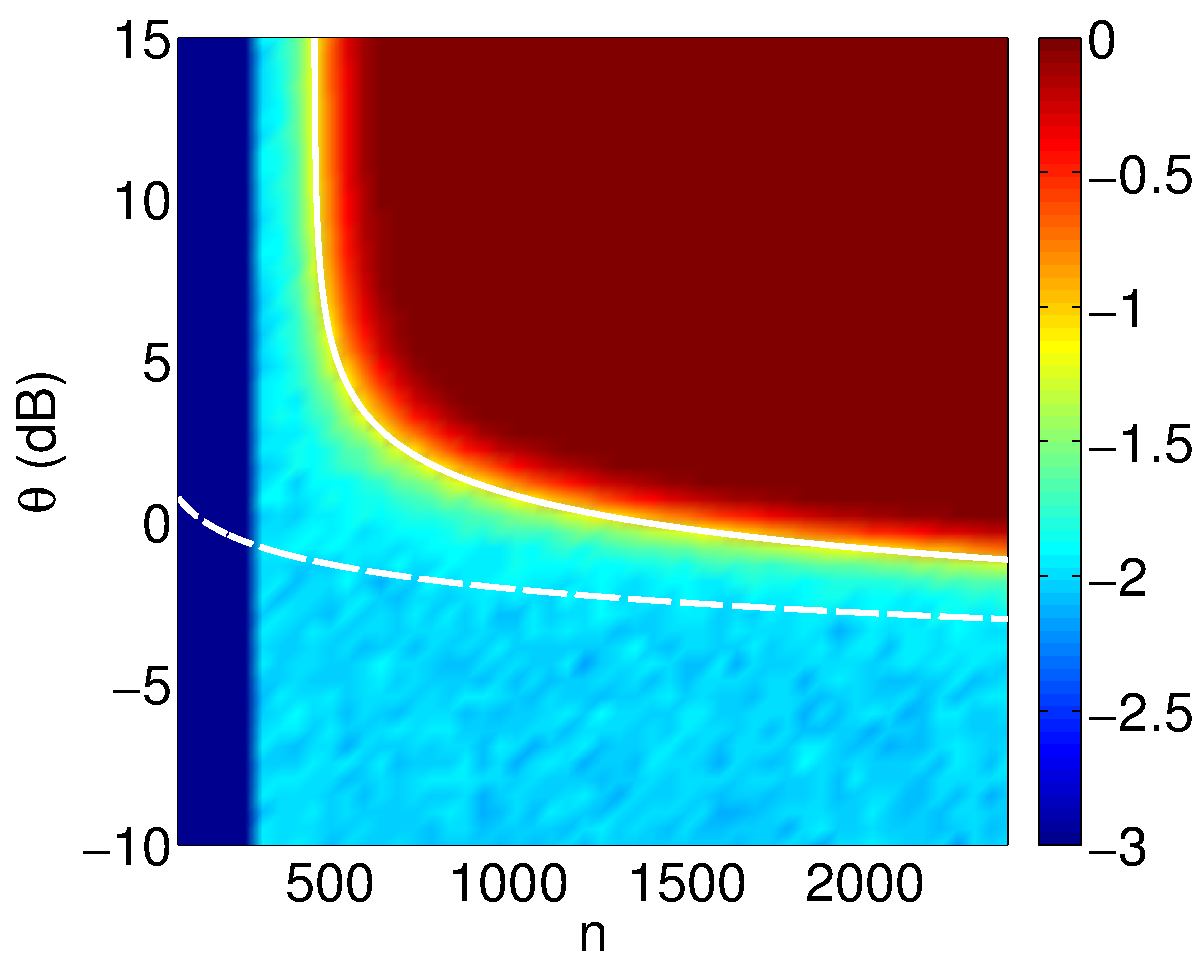
\includegraphics[width=0.4\textwidth]{figs/fig1a.pdf}
    }
    \subfigure[Empirical CCA $\rho=0.9$]{
      \label{fig:chpt4:cca_rho9}
      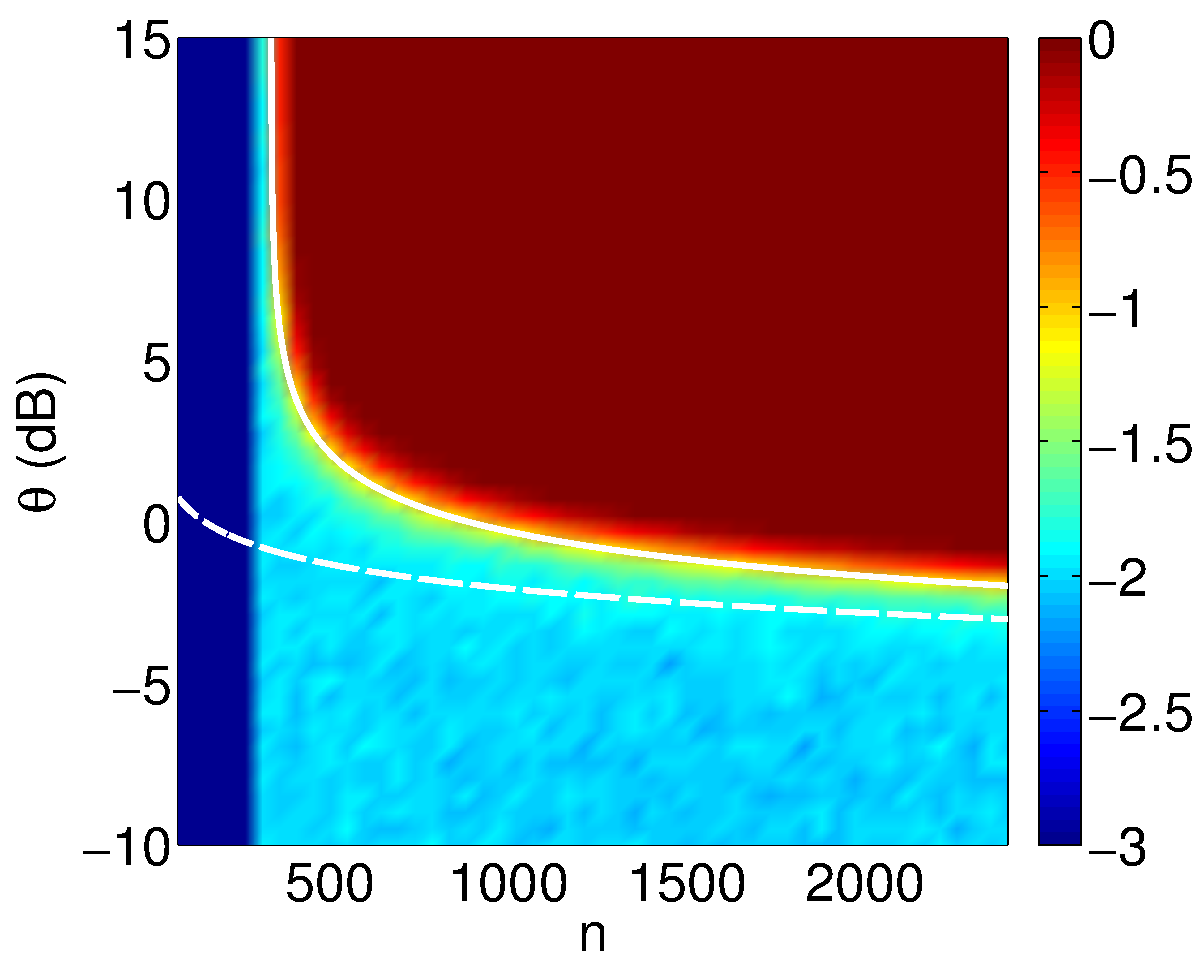
\includegraphics[width=0.4\textwidth]{figs/fig1b.pdf}
    }
    \subfigure[ICCA $\rho=0.7$]{
      \label{fig:chpt4:icca_rho7}
      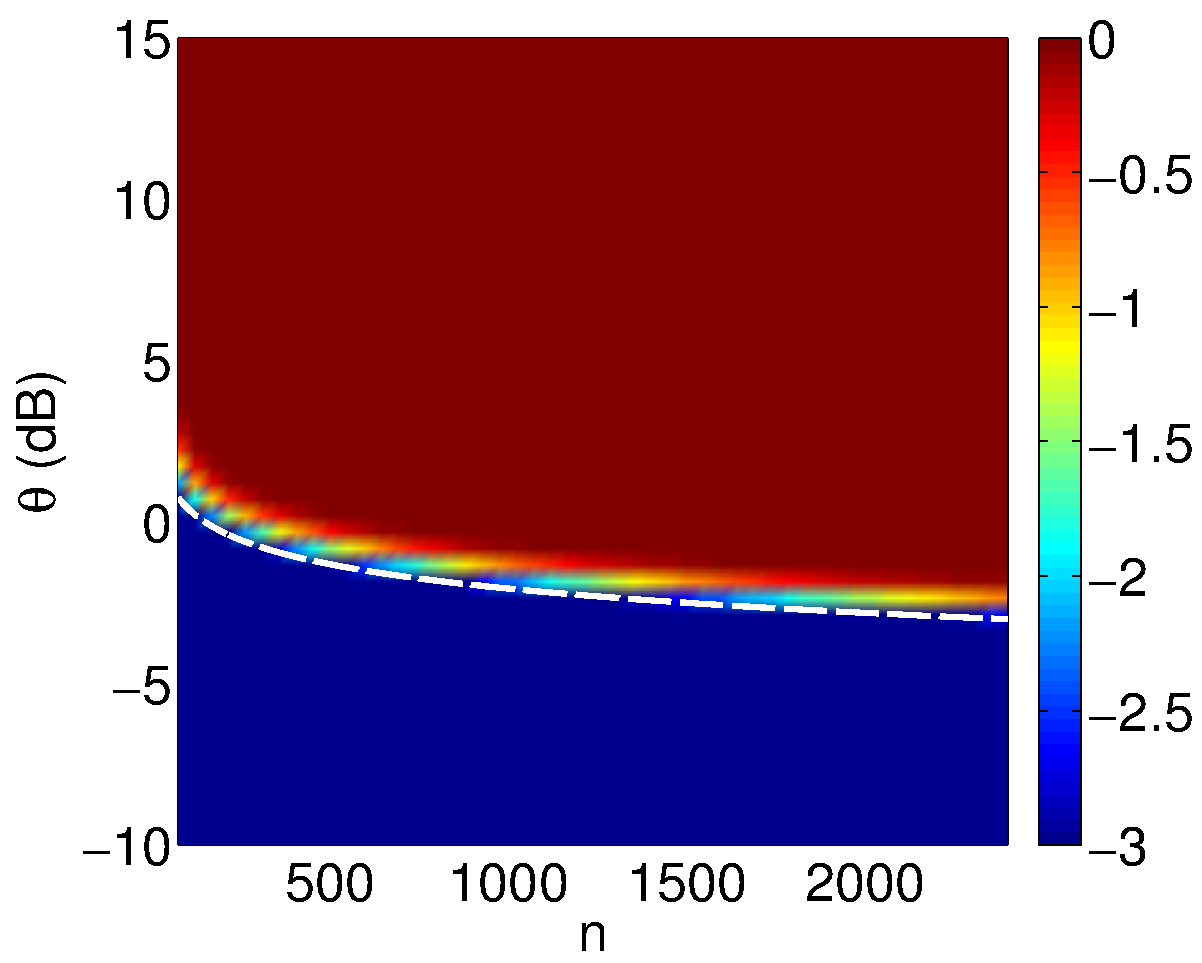
\includegraphics[width=0.4\textwidth]{figs/fig1c.pdf}
    }
    \subfigure[ICCA $\rho=0.9$]{
      \label{fig:chpt4:icca_rho9}
      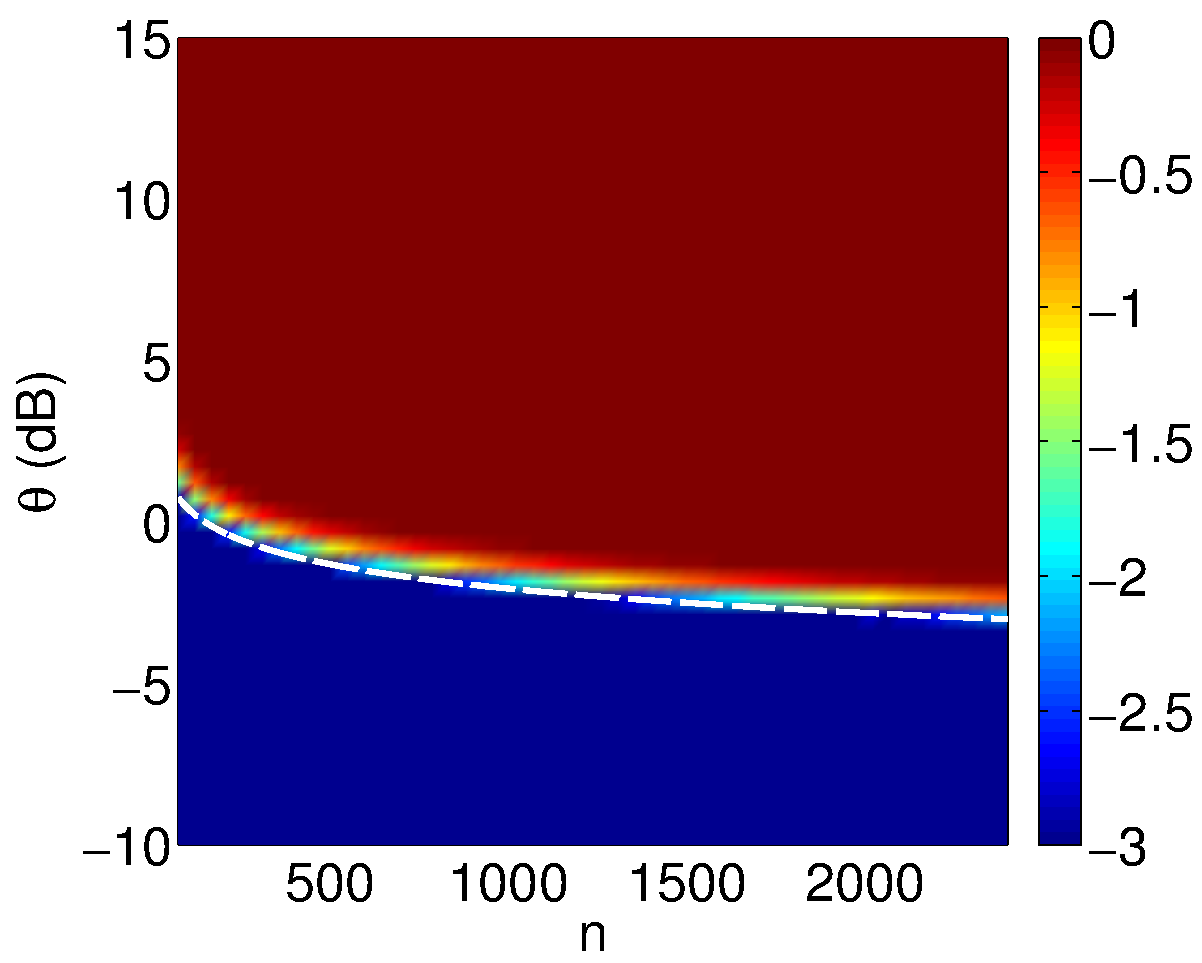
\includegraphics[width=0.4\textwidth]{figs/fig1d.pdf}
    }
    \caption{We generate data from (\ref{eq:chpt4:data_model}) for $p=q=150$, $\kx=\ky=1$,
      $k=1$, and various $\rho=\Pxy$ and sweep over $\theta = \tx_1=\ty_1$ and $n$. We
      compute $\kxhat$ and $\kyhat$ using Algorithm 2 of \cite{nadakuditi2010fundamental}
      for a significance value of $\alpha=0.01$. Using these estimates, we compute
      $\rhohatcca^{(1)}$ as the largest singular value of $\Cccahat$ as in
      (\ref{eq:chpt4:rhohatcca}) and $\rhohaticca^{(1)}$ as the largest singular value of
      $\Ciccahat$ as in (\ref{eq:chpt4:rhohaticca}). We then estimate the number of
      correlated signals $\khatcca$ and $\khaticca$ via (\ref{eq:chpt4:khats}) for a
      significance level of $\alpha=0.01$. We repeat this for 10000 trials and compute the
      percentage of trials where $\khatcca=1$ and $\khaticca=1$. We plot $\log_{10}$ of
      these percentages for multiples values of $\theta$ and $n$. We plot the theoretical
      phase transition of empirical CCA (given in Proposition \ref{prop:bao} that
      relies on \cite{bao2014canonical}) in a solid white line and the theoretical
      phase transition of ICCA (given in Theorem \ref{th:khat_lims}) in a dashed white
      line.}
    \label{fig:chpt4:cca_pt}
  \end{center}
\end{figure*}

Next, we explore the minimum $1/c$ for $c=c_x=c_y$ needed to reliably detect $k=1$
correlated signal in the experiment setting described for Figure
\ref{fig:chpt4:cca_pt}. As $c=p/n=q/n$, the minimum $1/c$ is equivalent to the minimum
number of samples needed for fixed dimensions. Using the theoretical phase transitions in
Proposition \ref{prop:bao} and Theorem \ref{th:khat_lims}, we have that this critical
value of $c$ is $c_{\text{crit}} = \theta^4$ for ICCA and $c_{\text{crit}} =
\min\left(\frac{r_c^{\text{crit}}}{1+r_c^{\text{crit}}}, 0.5\right)$ for empirical CCA,
where \be r_c^{\text{crit}} = \left(\frac{-\rho +
    \sqrt{\rho^2+4\theta^2\rho^2(1+\theta^2\rho^2)}}{2(1+\theta^2\rho^2)}\right)^2.  \ee
Figure \ref{fig:chpt4:contours} plots level sets of $c_{\text{crit}}$ for empirical CCA
and ICCA for various values of $\theta=\tx_1=\ty_1$ and $\rho=\Pxy$. Recall that if
$c>0.5$, empirical CCA fails entirely, so for comparison we only show contour lines for
$1/c=10$ and $1/c=3$.

From this figure, we once again observe that the performance of ICCA is independent of the
value of $\rho=\Pxy$, while the performance of empirical CCA is highly dependent on the
correlation. This figure allows us to showcase that ICCA is theoretically better than
empirical CCA in all parameter regimes as ICCA can achieve the same performance of
empirical CCA given fewer samples at a lower SNR.

\begin{figure}
  \begin{center}
    \subfigure[Empirical CCA]{
      \label{fig:chpt4:cca_contours}
      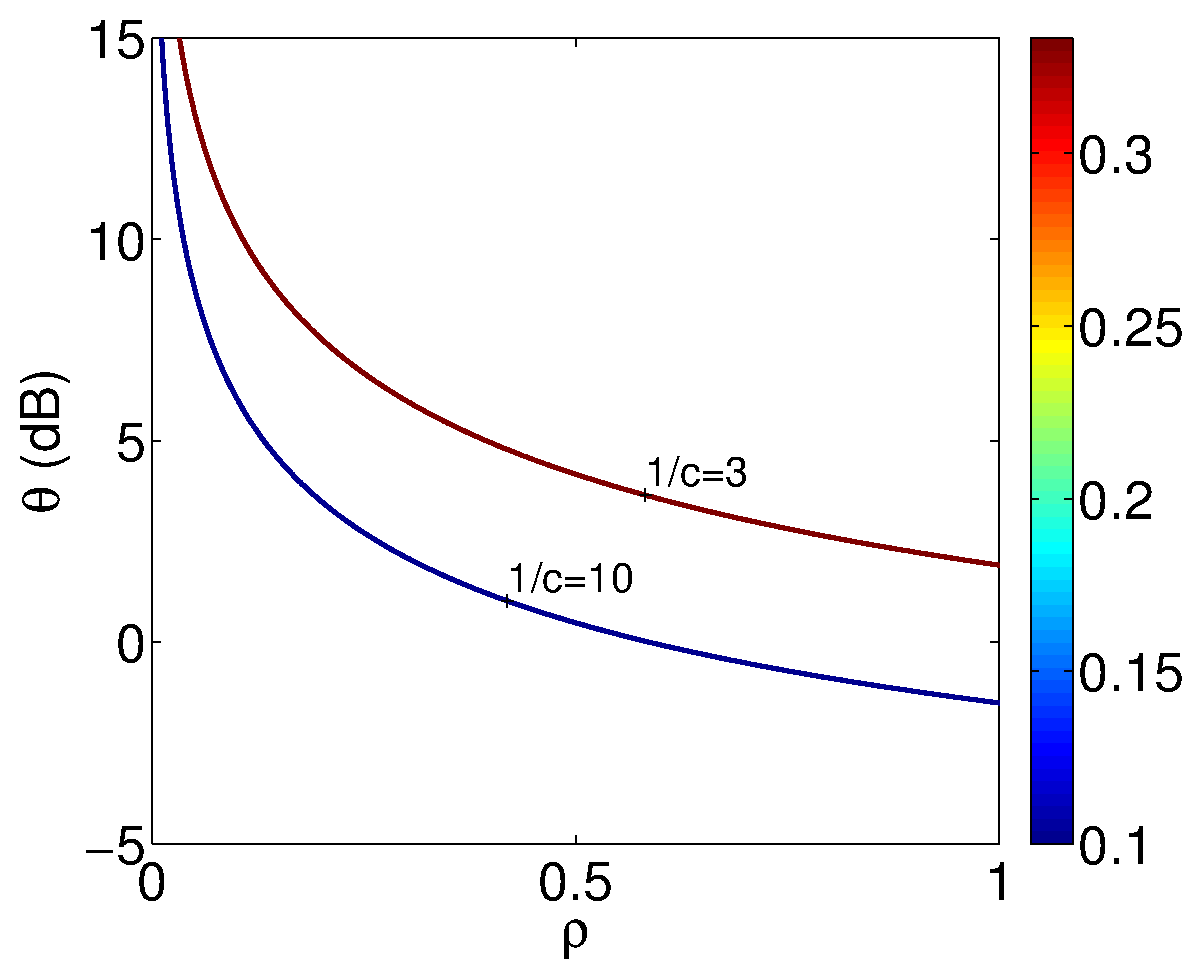
\includegraphics[width=0.4\textwidth]{figs/fig2a.pdf}
    }
    \subfigure[ICCA]{
      \label{fig:chpt4:icca_contours}
      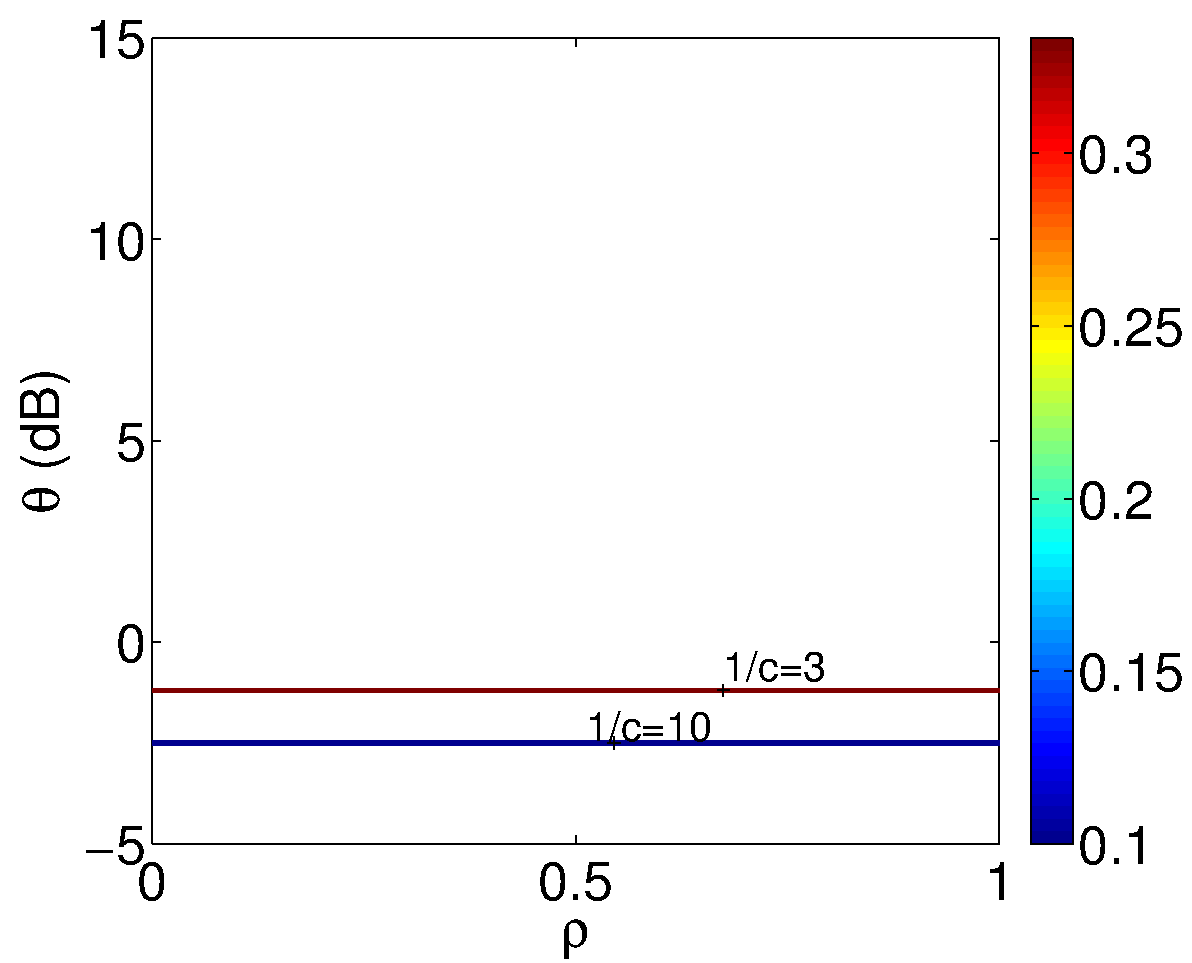
\includegraphics[width=0.4\textwidth]{figs/fig2b.pdf}
    }
    \caption{Contour lines for minimum $1/c$ necessary for reliable detection of $k=1$
      correlated component. The quantity $1/c = n/p$ is equivalent to the number of
      samples per dimension of data. For $c=c_x=c_y$, Figure \ref{fig:chpt4:cca_contours} plots the
      contours for empirical CCA using the limits given in Proposition \ref{prop:bao} and
      Figure \ref{fig:chpt4:icca_contours} plots the ICCA contours using the limits given
      in Theorem \ref{th:khat_lims}. We plot the contours for $1/c=10$ and
      $1/c=3$.  These plots clearly demonstrate that the ICCA limits are independent of
      $\rho=\Pxy$ while those for empirical CCA are highly dependent on $\rho=\Pxy$. For a fixed number of
      samples (fixed $c$), ICCA can reliably detect the presence of a correlated signal at
      lower SNR values than empirical CCA.}
    \label{fig:chpt4:contours}
  \end{center}
\end{figure}


\subsection{Simulated Missing Data}

Next, we demonstrate the accuracy of the performance limits for both empirical CCA and
ICCA in the setting of missing data described in Theorem \ref{th:missing_data} and
Conjecture \ref{conj:cca_missing}. Again, we consider a rank-1 setting ($\kx=\ky=1$) but
generate data from (\ref{eq:chpt4:data_model_miss}) for fixed $p=q=150$ over various
number of samples $n$, signal-to-noise ratio (SNR) $\theta=\tx_1=\ty_1$, various
$\rho=\Pxy$ (so that $k=1$), and also various percentages of missing data
$\gamma=\gamma_x=\gamma_y$. In all simulations, we use Algorithm 2 of
\cite{nadakuditi2010fundamental} to estimate $\kxhat$ and $\kyhat$ using a significance
level of $\alpha=0.01$. We stack the data into matrices $X$ and $Y$ and compute
$\rhohatcca^{(1)}$ and $\rhohaticca^{(1)}$ from the SVD of of $\Cccahat$ and $\Ciccahat$,
respectively. Using these correlation estimates, we compute the estimated number of
correlated components via (\ref{eq:chpt4:khats}) for a significance level of
$\alpha=0.01$. For a fixed set of parameters ($n$, $\theta$, $\rho$, $\gamma$) we repeat
the above process for 10000 trials and determine the percentage of trials where we detect
$\khatcca=1$ and $\khaticca=1$. Figure \ref{fig:chpt4:cca_missing_75} plots the
$\log_{10}$ of this percentage for empirical CCA and ICCA, respectively. We
overlay the ICCA performance boundary given by Theorem \ref{th:missing_data} in a dashed line
and the empirical CCA performance boundary given by Conjecture \ref{conj:cca_missing} in a
solid line.

From these figures, we observe that Theorem \ref{th:missing_data} and Conjecture
\ref{conj:cca_missing} accurately predict the phase transition for both empirical CCA and
ICCA in the presence of missing data for a wide array of parameters. Even in the presence
of missing data, ICCA can detect the presence of the correlated signal in the low-sample
regime ($n<p+q$) where empirical CCA deterministically fails.  In this missing data
setting, we once again observe that the value of $\rho$ affects the phase transition for
empirical CCA but not for ICCA; it is harder for CCA to detect signals with small
correlations.

\begin{figure*}
  \begin{center}
    \subfigure[Empirical CCA $\rho=0.7$]{
      \label{fig:chpt4:cca_rho3_75}
      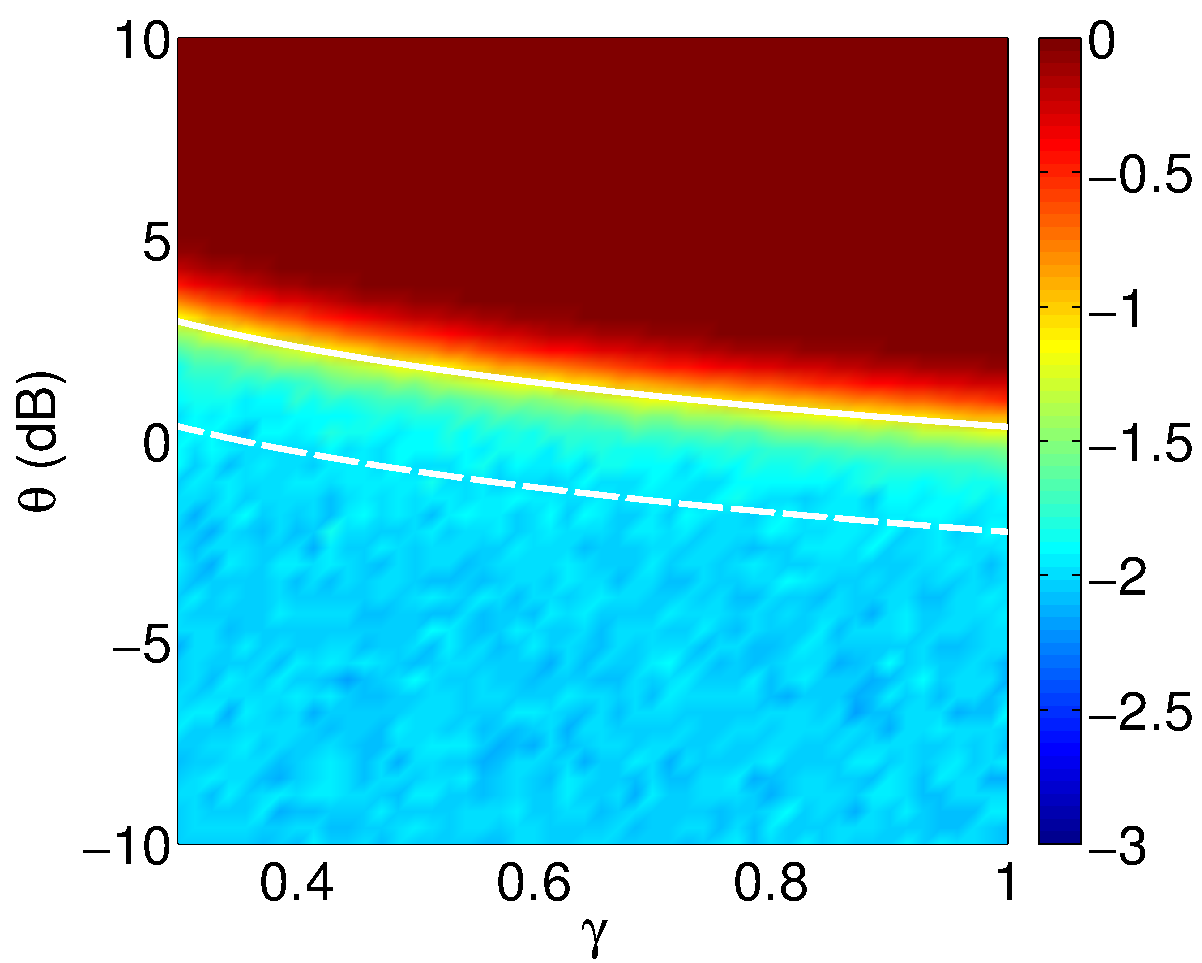
\includegraphics[width=0.4\textwidth]{figs/fig3a.pdf}
    }
    \subfigure[Empirical $\rho=0.9$]{
      \label{fig:chpt4:cca_rho5_75}
      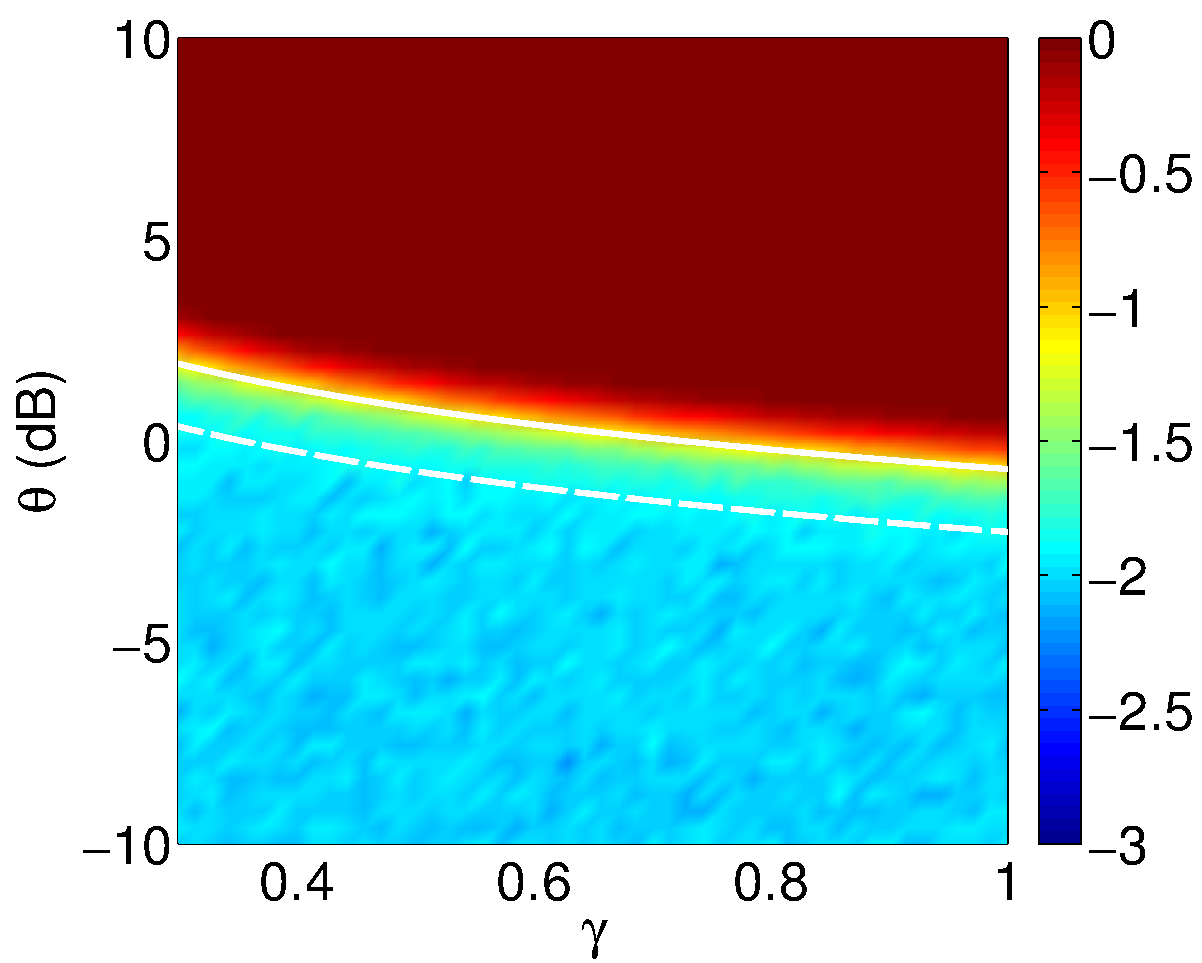
\includegraphics[width=0.4\textwidth]{figs/fig3b.pdf}
    }
    \subfigure[ICCA $\rho=0.7$]{
      \label{fig:chpt4:cca_rho7_75}
      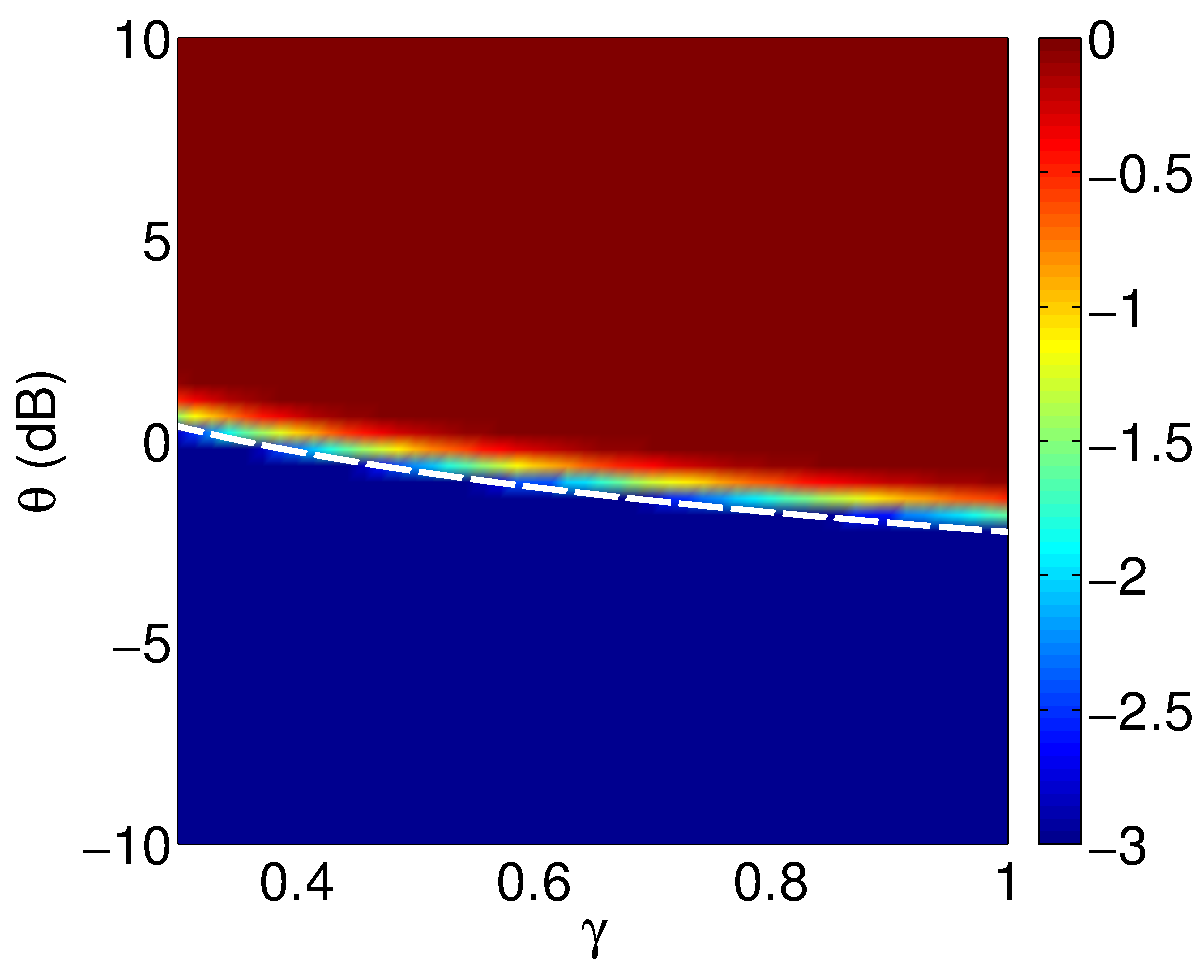
\includegraphics[width=0.4\textwidth]{figs/fig3c.pdf}
    }
    \subfigure[ICCA $\rho=0.9$]{
      \label{fig:chpt4:cca_rho9_75}
      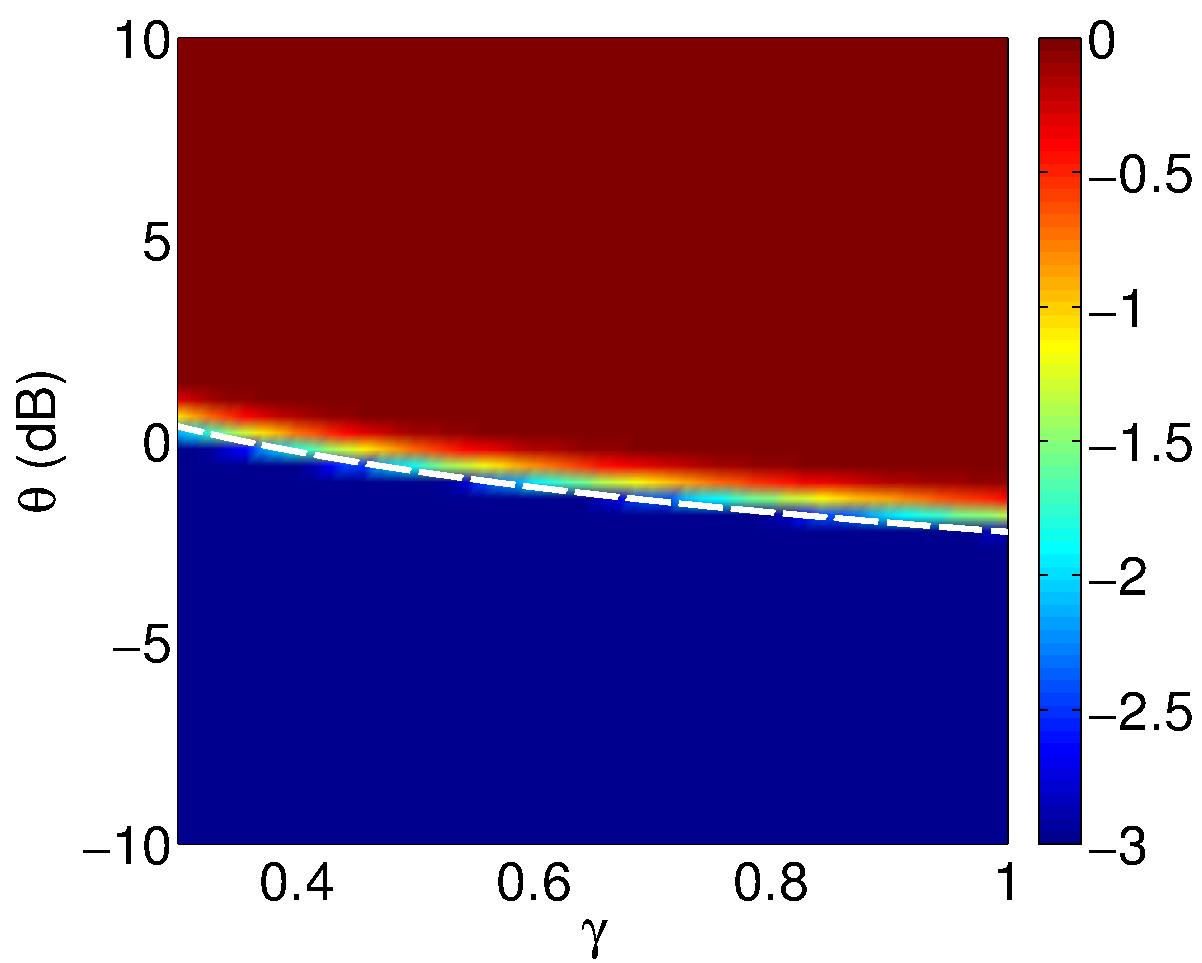
\includegraphics[width=0.4\textwidth]{figs/fig3d.pdf}
    }
    \caption{We generate data from (\ref{eq:chpt4:data_model_miss}) for $p=q=150$,
      $\kx=\ky=1$, $k=1$, $n=1200$, and various $\rho=\Pxy$ and sweep over $\theta =
      \tx_1=\ty_1$ and $\gamma=\gamma_x=\gamma_y$. We compute $\kxhat$ and $\kyhat$ as
      using Algorithm 2 of \cite{nadakuditi2010fundamental} for a significance value of
      $\alpha=0.01$. Using these estimates, we compute $\rhohatcca^{(1)}$ as the largest
      singular value of $\Cccahat$ as in (\ref{eq:chpt4:rhohatcca}) and
      $\rhohaticca^{(1)}$ as the largest singular value of $\Ciccahat$ as in
      (\ref{eq:chpt4:rhohaticca}). We then estimate the number of correlated signals
      $\khatcca$ and $\khaticca$ via (\ref{eq:chpt4:khats}) for a significance level of
      $\alpha=0.01$. We repeat this for 10000 trials and compute the percentage of trials
      where $\khatcca=1$ and $\khaticca=1$. We plot $\log_{10}$ of these percentages for
      multiples values of $\theta$ and $n$. We plot the theoretical performance limit of
      empirical CCA (given in Conjecture \ref{conj:cca_missing}) in a solid white line and
      the theoretical performance boundary of ICCA (given in Theorem
      \ref{th:missing_data}) in a dashed white line.}
    \label{fig:chpt4:cca_missing_75}
  \end{center}
\end{figure*}

\subsection{Controlled Flashing Lights Experiment}

To verify the effectiveness of ICCA for real world applications, we conducted a controlled
experiment consisting of 5 stationary flashing lights and two stationary iPhone
cameras\footnote{For a video demonstration of this experiment, visit
  \texttt{https://www.youtube.com/watch?v=WYlC2XgBDXs}. For similar experiments on an
  audio-audio dataset, visit \texttt{https://www.youtube.com/watch?v=lQzO10S7PEs} and an
  audio-video dataset visit\\ \texttt{https://www.youtube.com/watch?v=8E83P-\_oVgg}.}. Figure
\ref{fig:chpt4:flashing_sources} shows the left and right camera views at one time point
of our experiment and manually identifies each source. The 5 sources are a blue flashing
police light (BPL) outlined in the green rectangle, one phone with a flashing strobe light
(PH1) outlined in the dark blue rectangle, another phone with a flashing strobe light
(PH2) outlined in a red rectangle, a tablet with a flashing screen (T1) outlined in the
magenta rectangle, and a red flashing police light (RPL) outlined in the cyan
rectangle. From left to right, the left camera can see BPL, PH1, and PH2. From left to
right, the right camera can see PH2, T1, and RPL. Therefore, both cameras share the common
signal of PH2.

\begin{figure}
  \begin{center}
    \subfigure[Left Camera]{
      \label{fig:chpt4:flashing_left}
      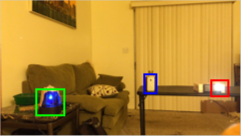
\includegraphics[width=0.47\textwidth]{figs/fig4a.png}
    }
    \subfigure[Right Camera]{
      \label{fig:chpt4:flashing_right}
      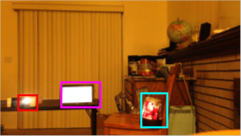
\includegraphics[width=0.47\textwidth]{figs/fig4b.png}
    }
    \caption{Left and right camera views of our experiment with boxes manually identifying
      each source. Both cameras share a common flashing phone, outlined in a red
      rectangle. Each camera has two independent sources besides the shared flashing
      phone.}
    \label{fig:chpt4:flashing_sources}
  \end{center}
\end{figure}


To synchronize the cameras we used the RecoLive MultiCam iPhone app
\footnote{http://recolive.com/en/}. After turning on all light sources, we recorded 30
seconds of video at 30 frames per second. The resolutions of the iPhone's cameras were
both $1920\times 1080$ pixels. To post-process the video data, we first converted the
video streams to grayscale and then downsampled each spatial dimension by a factor of 8,
resulting in a resolution of $240\times 135$. We then vectorized each image and stacked
the 900 frames into data matrices, both of dimension $32400 \times 900$. Finally, we
subtract the mean from each dataset so that we may run empirical CCA and ICCA on the
zero-mean datasets, $X_{\text{left}}$ and $Y_{\text{right}}$.

First, we run principal component analysis (PCA) on $X_{\text{left}}$ and
$Y_{\text{right}}$ to identify the number of signals in each dataset. We know from our
setup that each camera has 3 independent sources. Figure \ref{fig:chpt4:flashing_svs}
plots the singular values of $X_{\text{left}}$ and $Y_{\text{right}}$. However, PCA does
not provided any information about whether the identified signals are correlated across
cameras. To identify correlated pixels between the cameras, we run empirical CCA and ICCA
after each new video frame. For frame $\ell$, we construct the $32400\times\ell$
submatrices $X_{\text{left}}^\ell$ and $Y_{\text{right}}^\ell$ by taking the matrix of the
first $\ell$ original vectorized frames and zero meaning it. We then use these matrices as
the input to empirical CCA and ICCA. Using our knowledge of 3 sources present in each
camera, we set $\kxhat=\kyhat=3$. Figure \ref{fig:chpt4:flashing_corrs} plots the top 3
correlation coefficients returned by empirical CCA and ICCA over the first 800
frames. Intuitively, empirical CCA returns perfect correlation as we have only a few
frames but a large dimension (pixels).


\begin{figure}
  \begin{center}
    \subfigure[Left camera]{
      \label{fig:chpt4:ul1}
      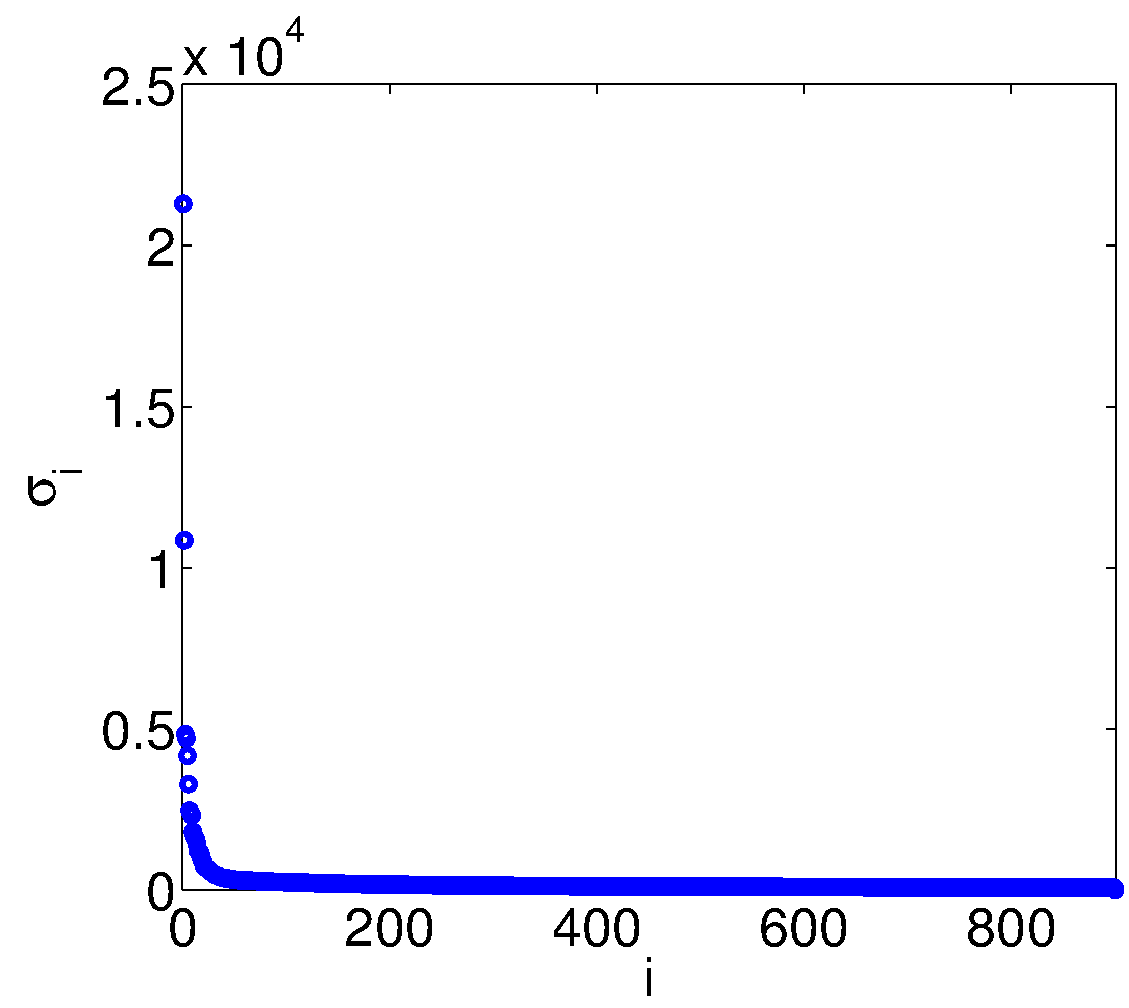
\includegraphics[width=0.4\textwidth]{figs/fig5a.pdf}
    }
    \subfigure[Right camera]{
      \label{fig:chpt4:ul2}
      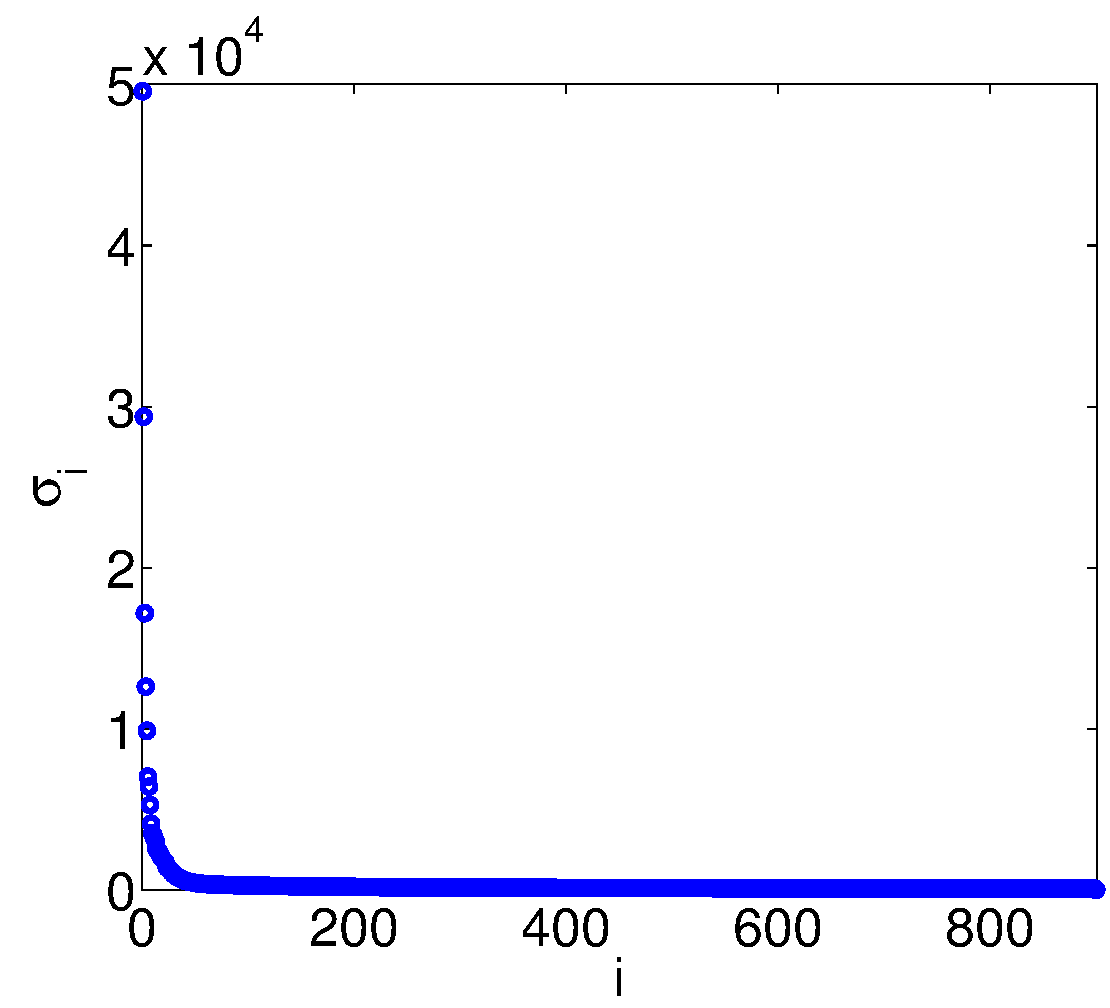
\includegraphics[width=0.4\textwidth]{figs/fig5b.pdf}
    }
    \caption{Singular value spectra of $X_{\text{left}}$ and $Y_{\text{right}}$ for the
      flashing light experiment.}
    \label{fig:chpt4:flashing_svs}
  \end{center}
\end{figure}


\begin{figure}
  \begin{center}
    \subfigure[CCA]{
      \label{fig:chpt4:flashing_cca_corrs}
      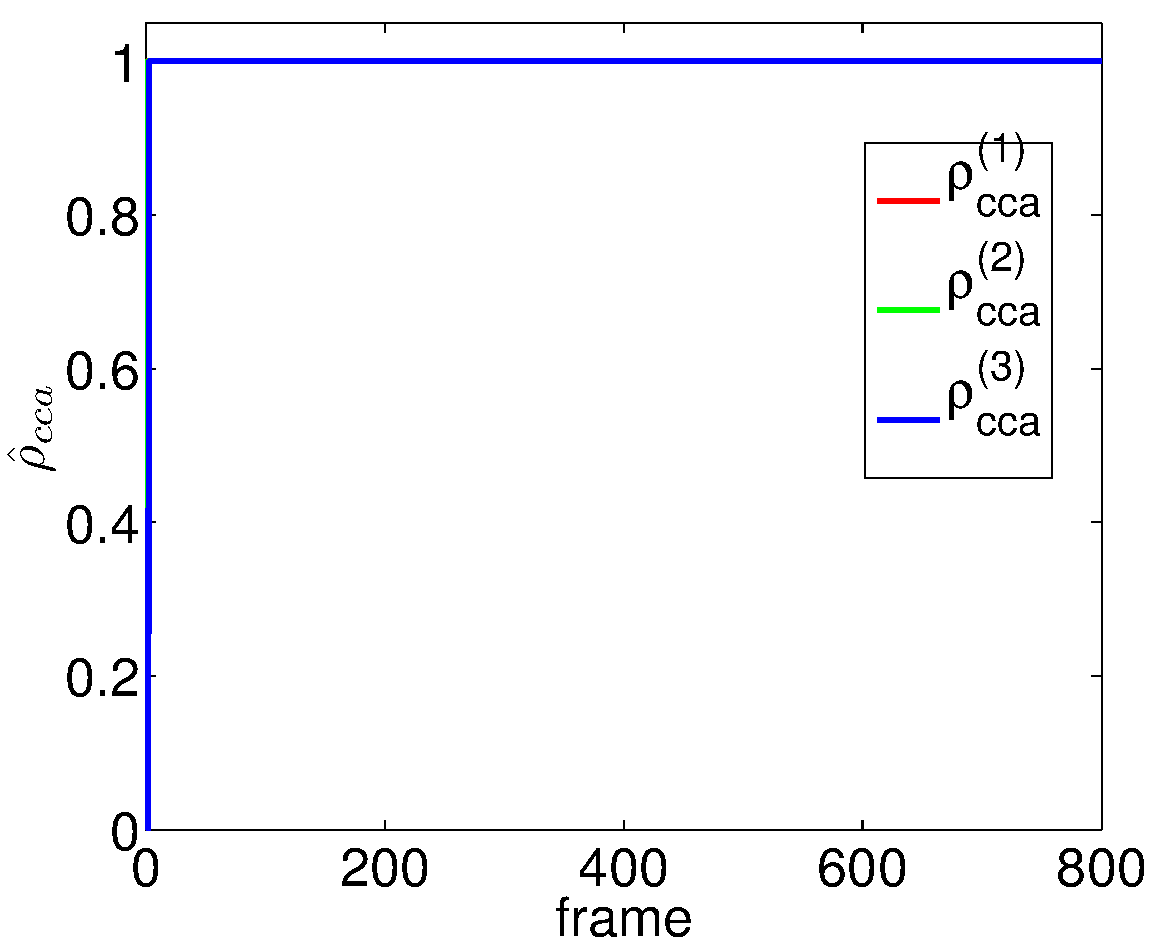
\includegraphics[width=0.4\textwidth]{figs/fig6a.pdf}
    }
    \subfigure[ICCA]{
      \label{fig:chpt4:flashing_icca_corrs}
      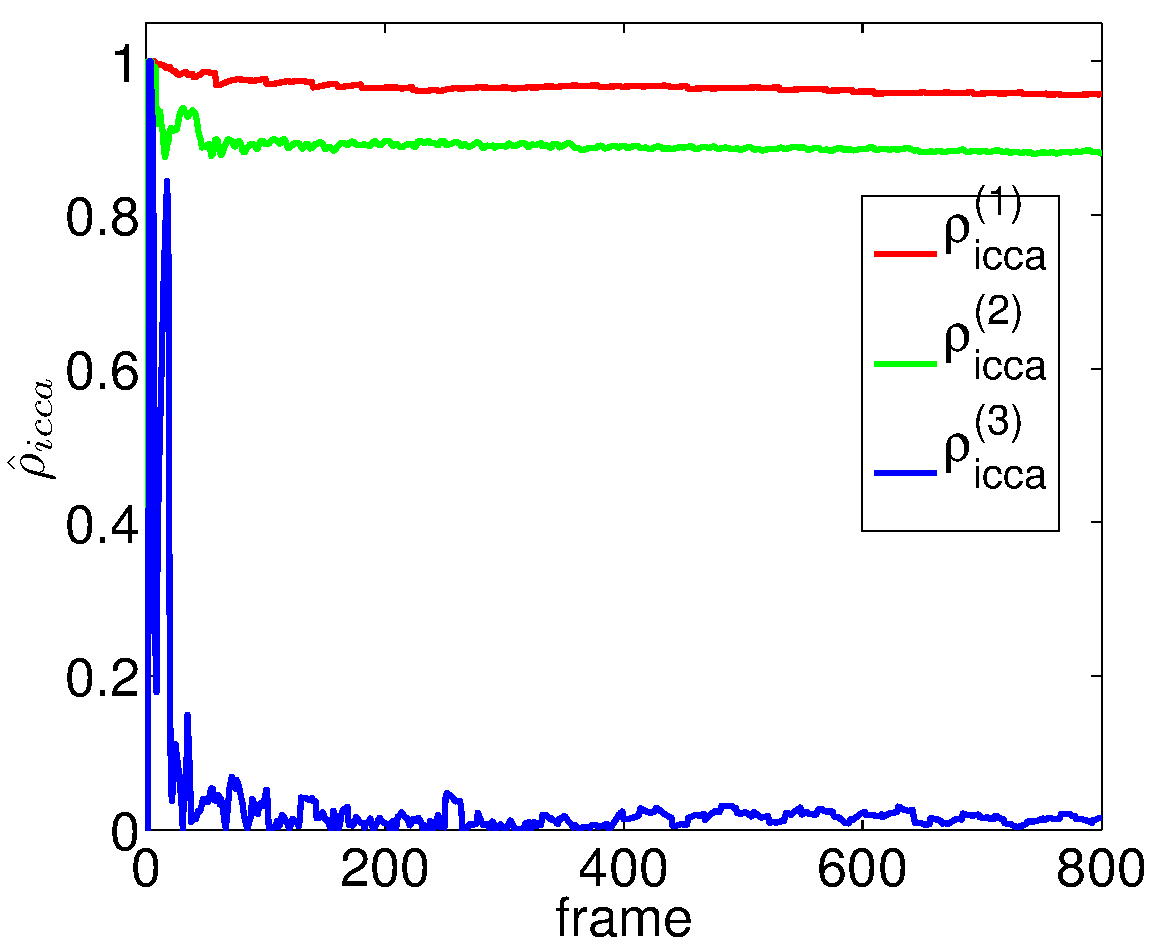
\includegraphics[width=0.4\textwidth]{figs/fig6b.pdf}
    }
    \caption{(a) Top three singular values returned by empirical CCA as defined in
      (\ref{eq:chpt4:rhohatcca}) for the flashing light demonstration. As we are in the
      sample deficient regime, these singular values are deterministically 1. (b) Top
      three singular values returned by ICCA as defined in (\ref{eq:chpt4:rhohaticca}) for
      the flashing light demonstration. ICCA correctly identifies two sources of
      correlation.}
    \label{fig:chpt4:flashing_corrs}
  \end{center}
\end{figure}

Using these singular values returned by empirical CCA and ICCA, we can set a threshold via
(\ref{eq:chpt4:taus}) to determine which ones indicate the presence of a correlated signal
between the datasets. Examining Figure \ref{fig:chpt4:flashing_corrs}, we can easily
accomplish this for ICCA as the top two singular values separate from the third. However,
as we operate in the sample deficient regime, we cannot set such a threshold for empirical
CCA to detect the presence of correlated signals. We overlay the thresholded unit-norm
canonical vectors (defined in (\ref{eq:chpt4:cca_vects}) and (\ref{eq:chpt4:icca_vects})) onto
the original images in Figure \ref{fig:chpt4:flashing_cca} for both empirical CCA and
ICCA. From this figure, we observe that the empirical CCA canonical vectors appear to be
very random and noisy. The ICCA canonical vectors correctly identify both sources of
correlation in our dataset.

\begin{figure}
  \begin{center}
    \subfigure[Left Camera - empirical CCA]{
      \label{fig:chpt4:flashing_left_cca}
      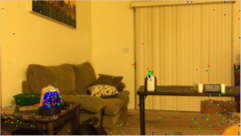
\includegraphics[width=0.4\textwidth]{figs/fig7a.png}
    }
    \subfigure[Right Camera - empirical CCA]{
      \label{fig:chpt4:flashing_right_cca}
      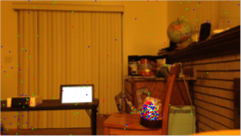
\includegraphics[width=0.4\textwidth]{figs/fig7b.png}
    }
    \subfigure[Left Camera - ICCA]{
      \label{fig:chpt4:flashing_left_icca}
      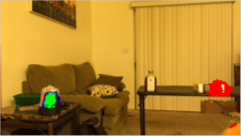
\includegraphics[width=0.4\textwidth]{figs/fig7c.png}
    }
    \subfigure[Right Camera - ICCA]{
      \label{fig:chpt4:flashing_right_icca}
      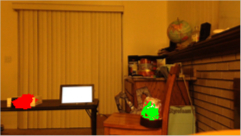
\includegraphics[width=0.4\textwidth]{figs/fig7d.png}
    }
    \caption{(a)-(b) Top 3 threholded empirical CCA canonical vectors overlayed on the
      original scene after 800 frames as computed in (\ref{eq:chpt4:cca_vects}). The red
      pixels correspond to the vector with the highest correlation, the green pixels
      correspond to the vector with the second highest correlation, and the blue pixels
      correspond to the vector with the third highest correlation in Figure
      \ref{fig:chpt4:flashing_cca_corrs}. We use a threshold of $\log(p)/\sqrt{p}$ where
      $p=32400$ pixels. (c)-(d) Top 2 threholded ICCA canonical vectors overlayed on video
      after 800 frames as computed in (\ref{eq:chpt4:icca_vects}). The red pixels
      correspond to the vector with the highest correlation and the green pixels
      correspond to the vector with the second highest correlation in Figure
      \ref{fig:chpt4:flashing_icca_corrs}. We again use a threshold of $\log(p)/\sqrt{p}$
      where $p=32400$ pixels.}
    \label{fig:chpt4:flashing_cca}
  \end{center}
\end{figure}

Given that our experiment setup has only one shared flashing light, it is initially
surprising that ICCA returns a two large singular values. Examining the ICCA canonical
vector overlay in Figure \ref{fig:chpt4:flashing_cca}, we observe that this correlation
corresponds to RPL and BPL. Figure \ref{fig:chpt4:flashing_v} examines the right singular
vectors returned by PCA corresponding to RPL and BPL. We observe that these light sources
have approximately the same period and even though they were started at random times, they
are in approximate antiphase, making them correlated. This is especially interesting
because neither camera can see both sources, but ICCA is still able to reveal a latent
correlation inherent in the period and phase of these lights.

\begin{figure}
  \begin{center}
      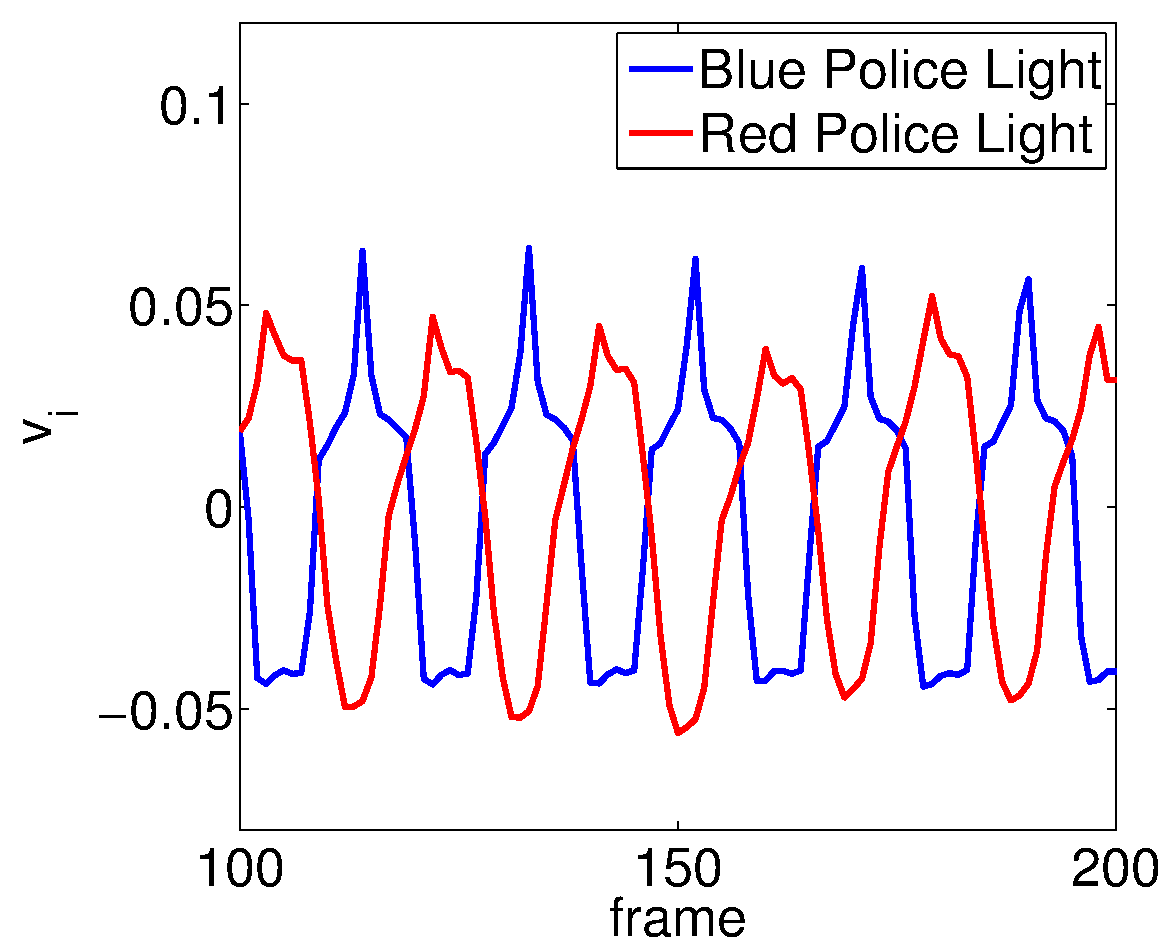
\includegraphics[width=0.4\textwidth]{figs/fig8.pdf}
    \caption{A portion of the right singular vectors of $X_{\text{left}}$ (blue) and
      $Y_{\text{right}}$ (red) corresponding the flashing police lights in each camera
      view. Both sources have very similar periods and are approximately in antiphase. }
    \label{fig:chpt4:flashing_v}
  \end{center}
\end{figure}

\subsection{Controlled Flashing Lights with Missing Data}

Using the same dataset in the previous section, we add missing data to each frame
independently\footnote{For a video demonstration of this experiment, please visit \texttt{https://www.youtube.com/watch?v=vhi3T4S8riE}}. We set $\gamma=\gamma_x=\gamma_y=0.75$ so that about 25\% of the pixels are
set to 0. We generate the missing pixels independently for each camera and for each
frame. We then process the data exactly as above without missing data. We note that in
this setup, our light sources do not obey the low-coherence condition, but we still run
ICCA to demonstrate its robustness. Particularly, source PH1 occupies only a small number
of pixels so that it has a very spiked signal and violates the low-coherence assumption
the most. In this missing data framework, PCA cannot detect this source. However, this
source is independent of all other signals as so we will still be able to detect all
correlated signal in the setting of Theorem \ref{th:missing_data}.

Figure \ref{fig:chpt4:flashing_cca_miss} overlays the thresholded canonical vectors
(defined in (\ref{eq:chpt4:cca_vects}) and (\ref{eq:chpt4:icca_vects})) corresponding to the
top 2 singular values for both empirical CCA and ICCA after 800 frames. Unsurprisingly,
empirical CCA is still unable to detect the two correlated signals because in this regime
the top singular values are deterministically one and the corresponding canonical vectors
are uninformative. However, ICCA is able to detect our correlated signals even in the
presence of missing data. The colored pixels clearly identify our two sources
of correlation.

\begin{figure}
  \begin{center}
    \subfigure[Left Camera - empirical CCA]{
      \label{fig:chpt4:flashing_left_cca}
      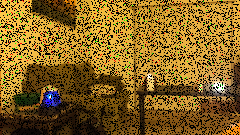
\includegraphics[width=0.4\textwidth]{figs/fig9a.png}
    }
    \subfigure[Right Camera - empirical CCA]{
      \label{fig:chpt4:flashing_right_cca}
      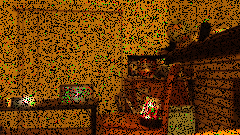
\includegraphics[width=0.4\textwidth]{figs/fig9b.png}
    }
    \subfigure[Left Camera - ICCA]{
      \label{fig:chpt4:flashing_left_icca_miss}
      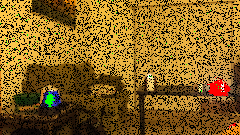
\includegraphics[width=0.4\textwidth]{figs/fig9c.png}
    }
    \subfigure[Right Camera - ICCA]{
      \label{fig:chpt4:flashing_right_icca_miss}
      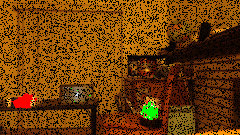
\includegraphics[width=0.4\textwidth]{figs/fig9d.png}
    }
    \caption{(a)-(b) Top 2 threholded empirical CCA canonical vectors overlayed on missing
      data video as computed in (\ref{eq:chpt4:cca_vects}). Again we use the threshold
      $\log(p)/\sqrt{p}$ for $p=32400$. The red pixels correspond to the vector with the
      highest correlation and the green pixels correspond to the vector with the second
      highest correlation in Figure \ref{fig:chpt4:flashing_cca_miss_svs}. (c)-(d) Top 2
      threholded ICCA canonical vectors overlayed on missing data video as computed in
      (\ref{eq:chpt4:icca_vects}). Again we use the threshold $\log(p)/\sqrt{p}$ for
      $p=32400$. The red pixels correspond to the vector with the highest correlation and
      the green pixels correspond to the vector with the second highest correlation in
      Figure \ref{fig:chpt4:flashing_cca_miss_svs}. For all figures,
      $\gamma_x=\gamma_y=0.75$ so that 25\% of our pixels are missing. We note that the
      middle source of the left camera violates the low-coherence assumption in Assumption
      \ref{assum:chpt4:coher} and so Theorem \ref{th:missing_data} and Conjecture
      \ref{conj:cca_missing} provide no guarantees for detecting correlations based on
      this source. }
    \label{fig:chpt4:flashing_cca_miss}
  \end{center}
\end{figure}

Figure \ref{fig:chpt4:flashing_corrs_miss} plots the top 3 singular values returned by
empirical CCA and ICCA. Unsurprisingly, the singular values reported by CCA are 1 and
uninformative. However, once we collect enough frames, there are two large singular values reported
by ICCA that identify the two sources of correlation in our dataset. Similar to the above
discussion, we can set a threshold via (\ref{eq:chpt4:taus}) to determine which ones
indicate the presence of a correlated signal between the datasets.

\begin{figure}
  \begin{center}
    \subfigure[Empirical CCA]{
      \label{fig:chpt4:flashing_cca_miss_svs}
      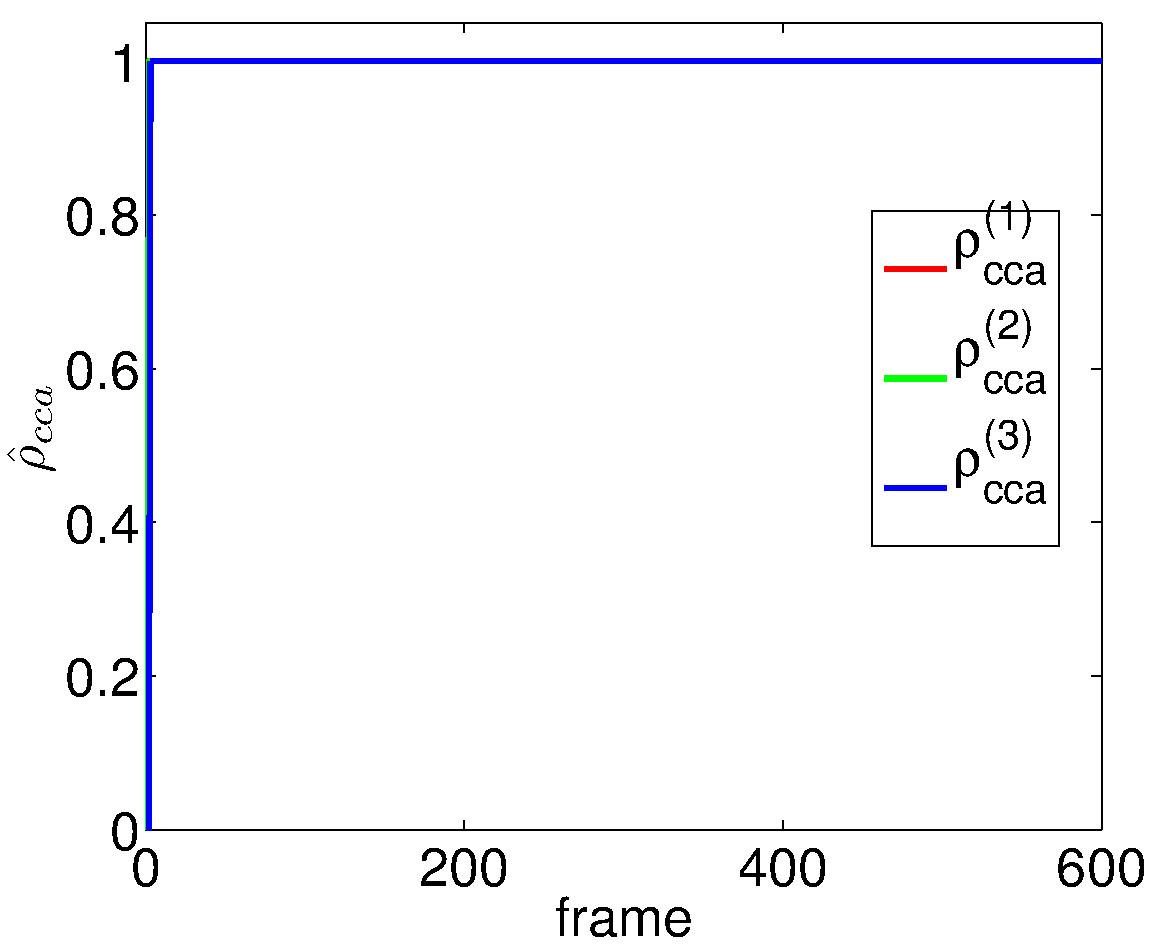
\includegraphics[width=0.4\textwidth]{figs/fig10a.pdf}
    }
    \subfigure[ICCA]{
      \label{fig:chpt4:flashing_icca_miss_svs}
      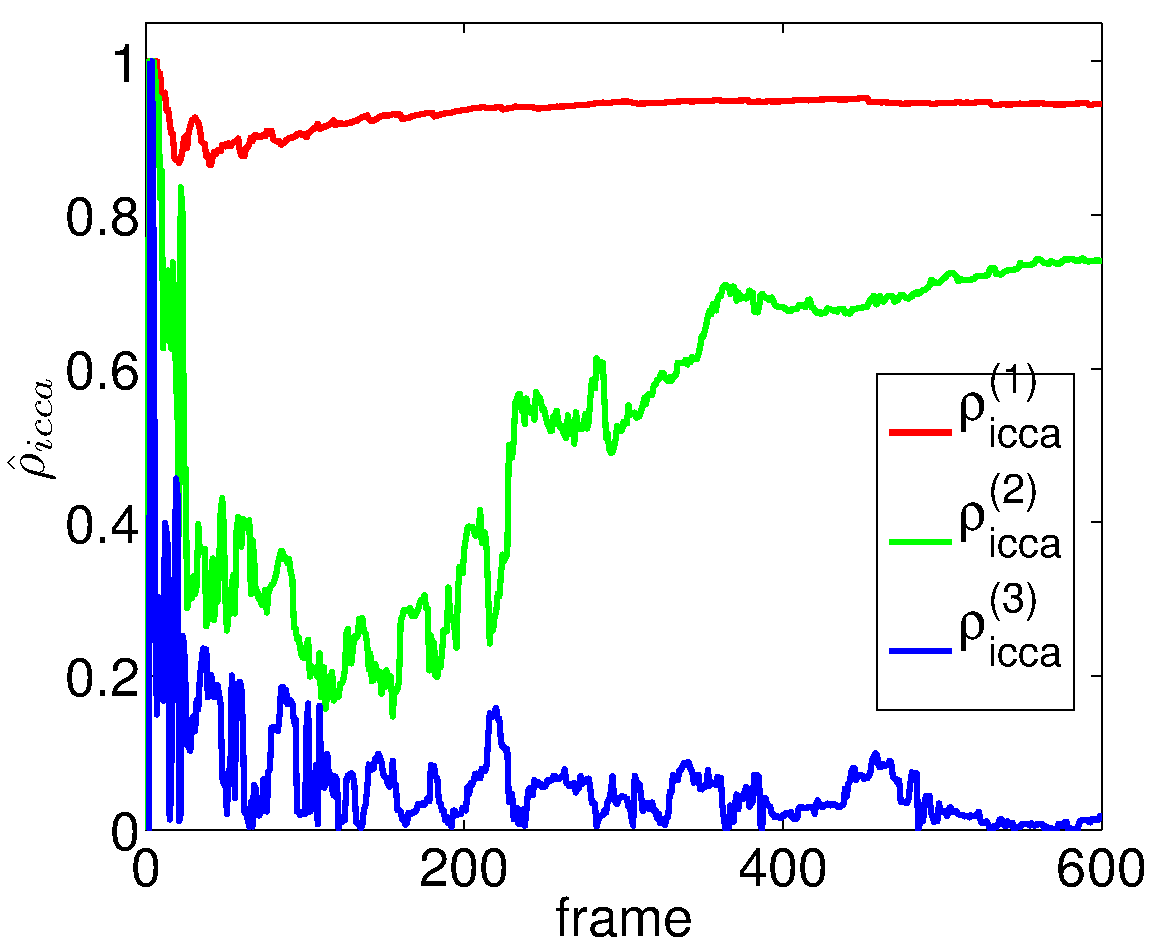
\includegraphics[width=0.4\textwidth]{figs/fig10b.pdf}
    }
    \caption{(a) Top three singular values returned by empirical CCA as defined in
      (\ref{eq:chpt4:rhohatcca}). As we are in the sample deficient regime, these singular
      values are deterministically 1. (b) Top three singular values returned by ICCA as
      defined in (\ref{eq:chpt4:rhohaticca}). ICCA correctly identifies two sources of
      correlation. As our data matrices now have missing data, it takes more frames for
      ICCA to identify the two sources of correlations. For both figures,
      $\gamma_x=\gamma_y=0.75$ so that 25\% of our pixels are missing. This figure is
      analogous to Figure \ref{fig:chpt4:flashing_corrs}, which observes all data so that
      $\gamma_x=\gamma_y=1$.}
    \label{fig:chpt4:flashing_corrs_miss}
  \end{center}
\end{figure}

\section{Conclusion}\label{sec:chpt4:concl}

In this paper we explored the problem of detecting correlations present in exactly two
datasets when the covariance and cross-covariance matrices are unknown and estimated from
training data. We showcased that the standard algorithm, empirical CCA, fails to detect
such correlations when the number of training samples is limited. Motivated by insights
from random matrix theory, we presented informative CCA (ICCA), which can reliably detect
correlations present in low-rank-correlated-signal-plus-noise type datasets. We then
extended this analysis to the case of missing data and showcased the improved detection
performance of ICCA on both synthetic and real-world examples. 

This paper assumed a low-rank-correlated-signal-plus-noise data model, which is ubiquitous
in signal processing applications.  We note that depending on the application, the linear,
low-rank-correlated-signal-plus-noise data model may be inappropriate. In such a setting,
kernel CCA (KCCA) \cite{welling2011first,yu2007learning} uses the kernel trick to first
map the data into a higher dimensional space before running CCA. The performance analysis
of such kernel methods for non-linear data models is important future
work. Proving Conjectures \ref{conj:khat_lims}, \ref{conj:icca}, and
  \ref{conj:cca_missing} remains an open problem and important area of future
  work. Finally, in a future paper we will characterize the accuracy of the empirical
  canonical vector estimates and provide a new estimate that uses insights from random
  matrix theory.


\appendix

\section*{Proof of Proposition \ref{prop:bao}}
Bao et al. \cite{bao2014canonical} proved this result for a slightly simplified
model. Here we provide the linear transformations to recover their model. We may write our
data matrices $X$ and $Y$ jointly via,
\be
\left[\begin{array}{c}X \\ Y\end{array}\right] = \left[\begin{array}{cc}\Rxx & \Rxy \\ \Rxy^H & \Ryy\end{array}\right]^{1/2}\left[\begin{array}{c}W_1 \\ W_2\end{array}\right]
\ee
where $W_1$ is a $p\times n$ matrix with independent $\mathcal{N}(0,1)$ entries and $W_2$
is an independent $q\times n$ matrix with independent $\mathcal{N}(0,1)$. As $p+q<n$,
$\Rxx$ and $\Ryy$ are non-singular. Define
{\small \be\ba
\left[\begin{array}{c}\widetilde{X} \\ \widetilde{Y}\end{array}\right] &=
\left[\begin{array}{cc}R_{xx}^{-1/2} & 0 \\ 0 &
    R_{yy}^{-1/2}\end{array}\right]^{1/2}\left[\begin{array}{c}X \\ Y\end{array}\right] \\
&=
\left[\begin{array}{cc}I_p & \Rxx^{-1/2}\Rxy\Ryy^{-1/2}.  \\ \Ryy^{-1/2}\Rxy^H\Rxx^{-1/2}
    & I_q\end{array}\right]\left[\begin{array}{c}W_1 \\ W_2\end{array}\right].
\ea\ee}
With the definitions of the covariance matrices in (\ref{eq:chpt4:true_scm}), we have that
$\Rxx^{-1/2}\Rxy\Ryy^{-1/2}$
\be\ba
&= \Ux\left(\Tx +
  I_{\kx}\right)^{-1/2}\Tx^{1/2}\Pxy\Ty^{1/2}\left(\Ty + I_{\ky}\right)^{-1/2}\Uy^H\\
 &= \Ux\Kxytil\Uy^H.
\ea\ee
From this expression, it is clear why we defined $\Kxytil$ as we originally did. Let
$U_{\Kxytil} K V_{\Kxytil}$ be the SVD of $\Kxytil$, where $K$ is the
$\kx\times\ky$ matrix with $\kappa_j$ along the diagonal. Define $F = \left[\left(\Ux
    U_{\Kxytil}\right) \,\,\,\left(\Ux U_{\Kxytil}\right)^{\perp}\right]$ and
$G=\left[\left(\Uy V_{\Kxytil}\right)\,\,\,\left(\Uy V_{\Kxytil}\right)^{\perp}\right]$. Then
\be\ba
&\left[\begin{array}{c}\widetilde{\widetilde{X}} \\ \widetilde{\widetilde{Y}}\end{array}\right] &&=
\left[\begin{array}{cc}F^H & 0 \\ 0 &
    G^H\end{array}\right]^{1/2}\left[\begin{array}{c}\widetilde{X} \\
    \widetilde{Y}\end{array}\right] \\ &&&=  \left[\begin{array}{cc}F^HR_{yy}^{-1/2} & 0 \\ 0 &
    G^HR_{yy}^{-1/2}\end{array}\right]^{1/2}\left[\begin{array}{c} X \\
    Y \end{array}\right]\\
&&& = \left[\begin{array}{cc}I_p & K \\ K^H &
    I_q\end{array}\right]^{1/2}\left[\begin{array}{c}W_1 \\ W_2\end{array}\right].
\ea\ee
Transforming $X$ and $Y$ to $\widetilde{\widetilde{X}}$ and
$\widetilde{\widetilde{Y}}$ preserves the canonical correlation estimates because our
transformation matrix is non-singular. After this transformation, we follow the proof from
Bao et al. \cite{bao2014canonical} with $\sqrt{r_i} = \kappa_i$.

\section*{Theorem needed to prove Theorem \ref{th:v_ip}}

\begin{Th}\label{th:w_ip}
Let $\widetilde{u}_i$ and $\widetilde{v}_i$ be the left and right singular vectors
associated with the $i$-th singular value, $\widetilde{\theta}_i$, of the $p\times n$ matrix
\be
\widetilde{X} = \sum_{i=1}^{k}\underbrace{\theta_i u_iv_i^H}_{P} + X.
\ee
Assume that $X$ satisfies
the hypotheses in Assumption \ref{assum:chpt4:noise} and suppose that $\theta_i>c^{1/4}$ for
$c=p/n$. Let $w$ be an
arbitrary unit norm vector that is orthogonal to $u_i$ for some $i\in\left\{1,\dots,k\right\}$. Then as $n,p\to\infty$ such that $p/n\to c$,  we have that
\be
\left\langle w,\widetilde{u}_i\right\rangle \convas 0.
\ee
\end{Th}
\begin{proof}
  The result of this theorem may be of interest outside of this paper for analysis of
  similar low-rank signal-plus-noise matrix models. We will use this theorem to prove
  Theorem \ref{th:v_ip}. We begin with a technical lemma needed to prove the theorem.

\begin{Lem}\label{lem:mip}
Let $U=[u_1,\dots,u_k]\in\complex^{p\times k}$ and $V=[v_1,\dots,v_k]\in\complex^{n\times
  k}$ be independent matrices with orthonormal columns. Let $X\in\complex^{p\times n}$
satisfy the hypotheses in Assumption \ref{assum:chpt4:noise}. Then as $n,p\to\infty$ with $p/n\to
c$, for $i\neq j$
\be
u_i^H\left(z^2 I_n - XX^H\right)^{-1}u_j \convas 0.
\ee
Similarly, for all $i,j$,
\be
u_i^H\left(z^2 I_n - XX^H\right)^{-1}Xv_j \convas 0.
\ee
\end{Lem}
\begin{proof}
The proof of Lemma 4.1 in \cite{benaych2012singular} proves both of these statements.
\end{proof}

We now are in a position to prove Theorem \ref{th:w_ip}. If $w\in\Span(u_1,\dots,u_k)$,
then Theorem 2.10 c) of \cite{benaych2012singular}
proves our result. If $w\not\in\Span(u_1,\dots,u_k)$, then we may write
\be
w = w_u + w_u^\perp,
\ee
where $w_u\in\Span(u_1,\dots,u_k)$ and $w_u^\perp$ is in the orthocomplement of
$\Span(u_1,\dots,u_k)$. Therefore applying Theorem 2.10 c) of \cite{benaych2012singular}
\be
\left\langle w,\widetilde{u}_i\right\rangle = \left\langle w_u,\widetilde{u}_i\right\rangle
+ \left\langle w_u^\perp,\widetilde{u}_i\right\rangle \convas \left\langle w_u^\perp,\widetilde{u}_i\right\rangle,
\ee
so we only must focus on $w_u^\perp$.

Based on their definitions, $\widetilde{X}\widetilde{X}^H\widetilde{u}_i =
\widetilde{\theta}_i^2\widetilde{u}_i$ and $\widetilde{X}^H\widetilde{u}_i =
\widetilde{\theta}_i\widetilde{v}$. Using the fact that $\widetilde{X}= P+X$, we have
\beq\label{eq:chpt4:step1}
\left(PP^H + PX^H + XP^H + XX^H\right)\widetilde{u}_i = \widetilde{\theta}_i^2\widetilde{u}_i
\eeq
and $\left(X^H+P^H\right)\widetilde{u}_i =\widetilde{\theta}_i\widetilde{v}$. Multiplying
both sides of this second expression by $P$, we have
\be
PX^H\widetilde{u}_i+PP^H\widetilde{u}_i =\widetilde{\theta}_iP\widetilde{v}_i.
\ee
Substituting this expression in (\ref{eq:chpt4:step1}) gives
\be
\widetilde{\theta}_iP\widetilde{v}_i +XP^H\widetilde{u}_i + XX^H\widetilde{u}_i =
\widetilde{\theta}_i^2\widetilde{u}_i .
\ee
Rearranging terms gives
\be
\widetilde{u}_i= \left(\widetilde{\theta}_i^2I_{p} -
  XX^H\right)^{-1}\left(\widetilde{\theta}_iP\widetilde{v}_i +XP^H\widetilde{u}_i\right).
\ee
Therefore, we have the equivalences for $\langle w_u^\perp,\widetilde{u}_i\rangle$
\be\ba
&=  &&w_u^{\perp H}\left(\widetilde{\theta}_i^2I_{p} -
  XX^H\right)^{-1}\left(\widetilde{\theta}_iP\widetilde{v}_i +XP^H\widetilde{u}_i\right)\\
& = &&\widetilde{\theta}_iw_u^{\perp H}\left(\widetilde{\theta}_i^2I_{p} -
  XX^H\right)^{-1}\sum_{j=1}^k\theta_j\langle v_j,\widetilde{v}_i\rangle u_j \\
&&&+
\widetilde{\theta}_iw_u^{\perp H}\left(\widetilde{\theta}_i^2I_{p} -
  XX^H\right)^{-1}X\sum_{j=1}^k\theta_j\langle u_j,\widetilde{u}_i\rangle v_j. \\
\ea\ee
By Theorem 2.7 c) in \cite{benaych2012singular}, we have that for $i\neq j$, $|\langle u_j,
\widetilde{u}_i\rangle|\convas 0 $ and $|\langle v_j, \widetilde{v}_i\rangle|\convas 0$. Therefore
\beq\label{eq:chpt4:w_thm_main}\ba
& \langle w_u^\perp,\widetilde{u}_i\rangle = &&\left(\widetilde{\theta}_i\theta_i\langle
  v_i,\widetilde{v}_i\rangle\right)w_u^{\perp H}\left(\widetilde{\theta}_i^2I_{p} -
  XX^H\right)^{-1} u_i \\
&&&+ \left(\widetilde{\theta}_i\theta_i\langle
  u_i,\widetilde{u}_i\rangle\right)w_u^{\perp H}\left(\widetilde{\theta}_i^2I_{p} -  XX^H\right)^{-1}X v_i. \\
\ea\eeq
By Lemma \ref{lem:mip},
\be
w_u^{\perp H}\left(\widetilde{\theta}_i^2I_{p} -  XX^H\right)^{-1} u_i\convas 0
\ee
and
\be
w_u^{\perp H}\left(\widetilde{\theta}_i^2I_{p} -  XX^H\right)^{-1}X v_i\convas 0.
\ee
Therefore, $\langle w_u^\perp,\widetilde{u}_i\rangle\convas 0$.
\end{proof}

\section*{Proof of Theorem \ref{th:v_ip}}
The entries of the matrix $\Vxcir^H\Vycir$ are the inner products between the columns of $\Vxcir$ and $\Vycir$
\be
\left|\left(\Vxcir^H\Vycir\right)\right|_{ij} = \left|\Vxcir^H(:,i)\Vycir(:,j)\right|.
\ee
Notice that we may write
\beq\label{eq:chpt4:v_orth}\ba
&\Vxcir(:,i) = a \Vy(:,j) + b w_y\\
&\Vy(:,j) = \kxy_{ij}\Vx(:,i) + c w_x
\ea\eeq
for some arbitrary unit-norm vector $w_x$ that is orthogonal to $\Vx(:,i)$, some arbitrary
unit-norm vector $w_y$ that is orthogonal to $\Vy(:,j)$, and constants $a$, $b$, and $c$. With
these observations, we have
\be\ba
& \Vxcir^H(:,i)\Vycir(:,j) && = \left(a \Vy(:,j) + b w_y\right)^H\Vycir(:,j)\\
&&& = a \Vy^H(:,j)\Vycir(:,j) + b w_y^H\Vycir(:,j).\\
\ea\ee
By Theorem \ref{th:w_ip}, $w_y^H\Vycir(:,j)\convas0$. As derived in theorem 5.2 in
\cite{nadakuditi2011fundamental},
{\small \be
\left|\Vy^H(:,j)\Vycir(:,j)\right|\convas\alpha_{y,j}\defeq\begin{cases} \sqrt{1 - \frac{c_y + \ty_j}{\ty_j(\ty_j + c_x)}} &
  \ty_j > c^{1/4} \\ 0 & \text{otherwise} \end{cases}.
\ee}
Therefore, $\left|\Vxcir^H(:,i)\Vycir(:,j)\right|\convas a\alpha_{y,j}$. Using the expression for
$\Vxcir(:,i)$ in (\ref{eq:chpt4:v_orth}), we observe that
\be
\Vy(:,j)^H\Vxcir(:,i) = a.
\ee
Using the expression for $\Vy(:,j)$ in (\ref{eq:chpt4:v_orth}), we have
\be\ba
& a  && = \Vy(:,j)^H\Vxcir(:,i)\\
&&& = \left(\kxy_{ij}\Vx(:,i) + c w_x\right)^H\Vxcir(:,i)\\
&&& = \kxy_{ij}\Vx^H(:,i)\Vxcir(:,i) + c w_x^H\Vxcir(:,i).\\
\ea\ee
By Theorem \ref{th:w_ip}, $w_x^H\Vxcir(:,i)\convas0$. As derived in theorem 5.1 of
\cite{nadakuditi2011fundamental},
{\small \be
\left|\Vy(:,j)\Vycir(:,j)\right|\convas\defeq\alpha_{x,i}\begin{cases} \sqrt{1 - \frac{c_x + \tx_i}{\tx_i(\tx_i + c_x)}} &
  \tx_i > c^{1/4} \\ 0 & \text{otherwise} \end{cases}.
\ee}
Therefore, $|a|\convas\left|\kxy_{ij}\right|\alpha_{x,i}$. Therefore,
\be
\left|\Vxcir^H(:,i)\Vycir(:,j)\right|\convas \left|\kxy_{ij}\right|\alpha_{x,i}\alpha_{y,i}.
\ee


\section*{Proof of Theorem \ref{th:khat_lims}}
For ICCA, recall that
\be
\khaticca = \sum_{i=1}^{\min(\kxhat,\kyhat)}
\indicator_{\left\{\left(\rhohaticca^{(i)}\right)^2 >\tauicca\right\}}.
\ee
When $\kxhat=\kx$ and $\kyhat=\ky$, the estimate of the number of correlated signals becomes
\be
\khaticca \convas \sum_{i=1}^{\min(\kx,\ky)} \indicator_{\left\{\left(\rhohaticca^{(i)}\right)^2 >\tauicca\right\}}.
\ee
To prove the theorem, we want to show that
\be
\rhohaticca^{(k)} > 0 \text{ almost surely},
\ee
under the conditions on $\Tx$ and $\Ty$ in the theorem statement. Momentarily, we assume that
$k=\min(\kx,\ky)$. The singular values of $\Vxcir^H\Vycir$ are
ordered and so we must show that 
\be
 \left(\rhohaticca^{(\min(\kx,\ky))}\right)^2 >\tauicca \text{ almost surely.}
\ee
From Theorem \ref{th:v_ip}, we also know that
\be
\left|\left[\Vxcir^H\Vycir\right]_{ij}\right| \convas\left|\kxy_{ij}\right|\alpha_{x,i}\alpha_{y,i}.
\ee
Using this fact we define
\be\ba
&A_x = \diag(\alpha_{x,1},\dots,\alpha_{x,\kx})\\
&A_y=\diag(\alpha_{y,1},\dots,\alpha_{y,\ky})\\
\ea\ee
so that we may write
\be
\Vxcir^H\Vycir = A_x\Kxy A_y + \Delta,
\ee
where $\Delta = [\delta_{ij}]$ such that $\delta_{ij} \convas 0$. Examining (\ref{eq:chpt4:alphas}), we see that under the above conditions on $\Tx$ and $\Ty$,
$A_x$ and $A_y$ are both full rank. Define
\be\ba
&\alpha_{x,\text{min}} = \min_{i=1\dots,\kx}\alpha_{x,i}\\
&\alpha_{y,\text{min}} = \min_{i=j\dots,\ky}\alpha_{y,j}.\\
\ea\ee
By properties of singular values
\be\ba
&\sigma_{\min}(A_x\Kxy A_y) - \sigma_{\max}(\Delta) &&\leq &&&\sigma_{\min}(A_x\Kxy A_y +
\Delta)\\ &&&\leq &&&\sigma_{\min}(A_x \Kxy A_y) \\ &&&&&&+ \sigma_{\max}(\Delta).
\ea\ee
Examining $\sigma_{\max}(\Delta)$, we observe that
\be
\sigma_{\max}(\Delta) \leq \|\Delta\|_F = \sqrt{\sum_{i=1}^{\kx} \sum_{j=1}^{\ky} \left|\delta_{ij}\right|^2}.
\ee
Using the fact that $\delta_{ij}\convas 0$, we have that $\sigma_{\max}(\Delta)\convas
0$. Therefore, almost surely
\be
\sigma_{\min}(A_x\Kxy A_y) \leq \sigma_{\min}(A_x\Kxy A_y +
\Delta)\leq \sigma_{\min}(A_x \Kxy A_y),
\ee
which implies that
\be
\rhohaticca^{(\min(\kx,\ky))}\convas\sigma_{\min}(A_x \Kxy A_y)
\ee
By properties of singular values
\be\ba
&\rhohaticca^{(\min(\kx,\ky))} && = \sigma_{\min(\kx,\ky)}\left(\Vxcir^H\Vycir\right)\\
&&& \convas \sigma_{\min(\kx,\ky)}\left(A_x\Kxy A_y\right)\\
&&& \geq \sigma_{\kx}\left(A_x\right)\sigma_{\min(\kx,\ky)}
\left(\Kxy\right)\sigma_{\ky}\left(A_y\right)\\
&&& = \alpha_{x,\text{min}}\kappa_{\min(\kx,\ky)}\alpha_{y,\text{min}} > 0,\\
\ea\ee
and we have proved the desired result.

\begin{comment}
Next we turn to our statistical test in the asymptotic setting. Unlike $\Cccahat$, whose
dimension scales with $n$, the dimension of $\Ciccahat$ remains $\kx\times\ky$ even as $n$
increases. Therefore, in the null setting as $n\to\infty$ the entries $\Ciccahat$ converge
almost surely to 0. Therefore, in the asymptotic setting our test becomes
\be
\khaticca = \sum_{i=1}^{\min(\kx,\ky)} \indicator_{\left\{\left(\rhohaticca^{(i)}\right)^2 >0\right\}}.
\ee
Therefore,
\be\ba
&\Prob{\left(\khaticca = k\right)} &&= \Prob{\left(\rhohaticca^{(\min(\kx,\ky))}\right)^2
  > 0 }\\
&&& \geq \Prob{\left(\alpha_{x,\text{min}}\kappa_{\min(\kx,\ky)}\alpha_{y,\text{min}}\right)^2  > 0 }\\
&&& \to 1.\\
\ea\ee
The last equality comes from the fact that under our conditions on $\Tx$ and $\Ty$,
the $\alpha$ terms are non-zero and from the fact that we momentarily assumed
$k=\min(\kx,\ky)$ so that $\kappa_{\min(\kx,\ky)}$ is non-zero. We note that this holds
for all significance levels.

Lastly, we argue that the above analysis holds when $k<\min(\kx,\ky)$. In this setting,
the last $\min(\kx,\ky)-k$ singular values of $A_y\Kxy A_y$ are zero. The above
analysis holds for the largest $k$ canonical correlations, showing that they are non-zero
in the asymptotic limit. Therefore, the asymptotic statistic will correctly mark these top $k$
singular values as an indicator of the $k$ correlations and correctly identify the
smallest $\min(\kx,\ky)-k$ singular values as not containing correlation as they are zero
in the asymptotic limit.
%Therefore,
%\be
%\Prob{\khaticca = k} \geq
%\Prob{\left(\alpha_{x,\text{min}}\kappa_{\min(\kx,\ky)}\alpha_{y,\text{min}}\right)^2 > \tauicca}.
%\ee
%Finally we examine $\tauicca$ when $p,q,n\to\infty$ with $p/n\to c_x$, $q/n\to c_y$ and
%$\kx$ and $\ky$ fixed. In the equations for $\mu_{\kx,\ky,n}$, we see that in this
%asymptotic setting, $\gamma\to 0$ and $\varphi\to 0$. Therefore
%$\mu_{\kx,\ky,n}\to\log(0)=-\infty$. Similarly, $\sigma_{\kx,\ky,n}\to c_\sigma$ for some
%finite $c_\sigma$ dependent on $\kx$ and $\ky$. Therefore, for all values of $\alpha$,
%\be
%\tauicca\to-\infty.
%\ee
%Therefore
%\be\ba
%&\Prob{\khaticca = k} &&\geq
%\Prob{\left(\alpha_{x,\text{min}}\kappa_{\min(\kx,\ky)}\alpha_{y,\text{min}}\right)^2 >
%  \tauicca}\\
%&&& \convas \Prob{\left(\alpha_{x,\text{min}}\kappa_{\min(\kx,\ky)}\alpha_{y,\text{min}}\right)^2 >
%  -\infty}
%&&& = 1.
%\ea\ee
%As $\alpha_{x,\text{min}}$, $\alpha_{y,\text{min}}$ and $\kappa_{\min(\kx,\ky)}$ are
%constant when $p,q,n\to\infty$ with $p/n\to c_x$, $q/n\to c_y$ and
%$\kx$ and $\ky$ fixed, we have that
%\be
%\Prob{\khaticca=k}\convas 1.
%\ee

\end{comment}

\section*{Proof of Theorem \ref{th:missing_data}}
Defining $P_x=\Ux\Vx^H$ We may write (\ref{eq:chpt4:data_model_miss}) as
\be\ba
& X &&= \underbrace{P_x\odot M_x}_{\widehat{P}_x} + \underbrace{Z_x\odot
  M_x}_{\widehat{Z}_x}\\
&&& = \E{\widehat{P}_x} + \widehat{Z}_x + \Delta_{\widehat{P}_x}\\
&&& = \underbrace{\gamma_x P_x + \widehat{Z}_x}_{\widetilde{X}} + \Delta_{\widehat{P}_x}.\\
\ea\ee
Similarly, we may write $Y=\widetilde{Y} + \Delta_{\widehat{P}_y}$ where $\widetilde{Y} =
\gamma_y P_y + \widehat{Z}_y$.

First we show that the maximum singular value of $\Delta_{\widehat{P}_x}$ and
$\Delta_{\widehat{P}_y}$ converge almost surely to 0. Under the low-coherence assumption,
we have that
\beq\ba\label{eq:chpt4:P}
&\max_{ij}|P_x|_{ij}&&\leq \max_{i}\tx_i\max_{k}\|u_k^{(x)}\|_\infty\max_{\ell}\|v_\ell^{(x)}\|_\infty\\ &&&=
  \max_{i}\tx_i\mathcal{O}\left(\frac{\text{log } n,p \text{ factors}}{\sqrt{np}}\right).
\ea\eeq
By assumption that $c_x>0$, we have that $n=\mathcal{O}(p)$. This fact, coupled with the
fact that $\tx_i$ is not dependent on $n$ gives
\beq\label{eq:chpt4:P_2}
\max_{ij}|P_x|_{ij}\leq \mathcal{O}\left(\frac{\text{log } n \text{ factors}}{n}\right).
\eeq
To characterize the largest singular value of $\Delta_{\widehat{P}_x}$, we want to use
Latala's theorem \cite{latala2005some}, which states that for a matrix $A$ with
independent mean zero random entries with bounded fourth moment
\be\ba
&\E{\sigma_1\left(A\right)} \leq
&&C\left[\max_i\left(\sum_j\E{A_{ij}^2}\right)^{1/2}\right . \\
  &&& +
    \max_j\left(\sum_i\E{A_{ij}^2}\right)^{1/2} \\
&&&\left . + \left(\sum_{i,j}\E{A_{ij}^4}\right)^{1/4}\right]
\ea\ee
for some universal constant $C$ that does not depend on $n$ or $p$. Through basic
calculation, one can show that
\be\ba
& \E{\left(\Delta_{\widehat{P}_x}\right)_{ij}^2} = \gamma_x\left(1-\gamma_x\right)\left(P_x\right)_{ij}^2\\
&\E{\left(\Delta_{\widehat{P}_x}\right)_{ij}^4} = \left(-3\gamma_x^4+6\gamma_x^3 -
  4\gamma_x^2 + \gamma\right)\left(P_x\right)_{ij}^4.\\
\ea\ee
These expressions satisfy the conditions on Latala's theorem. Therefore, by substituting
these expressions into Latala's theorem with the bound in (\ref{eq:chpt4:P_2}), we have
\be
\E{\sigma_1\left(\Delta_{\widehat{P}_x}\right)}\leq\mathcal{O}\left(\frac{\text{log } n \text{ factors}}{\sqrt{n}}\right).
\ee
By concentration and convexity of the largest singular value (see
\cite{nadakuditi2014optshrink} page 3015), we have that in our
asymptotic regime
\be
\sigma_1(\Delta_{\widehat{P}_x})\convas 0.
\ee
Using a similar argument
\be
\sigma_1(\Delta_{\widehat{P}_y})\convas 0.
\ee
Therefore we have that
\be\ba
&X\to \gamma_x P_x + \widehat{Z}_x\\
&Y\to\gamma_y P_y + \widehat{Z}_y.\\
\ea\ee
Examining $\widehat{Z}_x$, we have
\be\ba
&\E{\widehat{Z}_{ij}^{(x)}} =
&&\E{\widehat{Z}_{ij}^{(x)}|M_{ij}^{(x)}=0}\Prob{M_{ij}^{(x)}=0} \\
&&&+
\E{\widehat{Z}_{ij}^{(x)}|M_{ij}^{(x)}=1}\Prob{M_{ij}^{(x)}=1} = 0
\ea\ee
and
\be\ba
\E{\left(\widehat{Z}_{ij}^{(x)}\right)^2} &=
&&\E{\left(\widehat{Z}_{ij}^{(x)}\right)^2|M_{ij}^{(x)}=0}\Prob{M_{ij}^{(x)}=0}+ \\
&&&
\E{\left(\widehat{Z}_{ij}^{(x)}\right)^2|M_{ij}^{(x)}=1}\Prob{M_{ij}^{(x)}=1}\\
& = &&0 + \gamma_x.
\ea\ee
Therefore, $\widehat{Z}_{ij}^{(x)}$ are i.i.d. zero mean with variance
  $\gamma_x$ and $\widehat{Z}_x\to\sqrt{\gamma_x}Z_x$. Using this observation,
\be\ba
&X &&\convas \gamma_x P_x + \widehat{Z}_x\\
&&& \to \gamma_x P_x + \sqrt{\gamma_x}Z_x\\
&&& = \sqrt{\gamma_x}\left(\sqrt{\gamma_x} P_x + Z_x\right).\\
\ea\ee
Similarly, $Y\to\sqrt{\gamma_y}\left(\sqrt{\gamma_y} P_y + Z_y\right)$.

From this we can conclude that eigenvector expressions of the form $\langle u, \widehat{u}\rangle$
behave as if we replace $\Tx$ with $\gamma_x\Tx$ and $\Ty$ with $\gamma_y\Ty$. Consider
\beq\label{eq:chpt4:ip_missing_orig}\ba
&\left|u_i^H\left(zI - (Z_x + \Delta_{\widehat{P}_x}) \right. \right .&&\left . (Z_x +
  \Delta_{\widehat{P}_x})^H\right)^{-1} \cdot \\  &&& \left. u_j - u_i^H\left(zI - Z_xZ_x^H\right)^{-1}u_j
\right|,
\ea\eeq
which as a consequence of the variational characterization of the largest singular value
is upper bounded by
{\small \beq\label{eq:chpt4:ip_missing}
\sigma_1\left(\left(zI - (Z_x + \Delta_{\widehat{P}_x})(Z_x +
  \Delta_{\widehat{P}_x})^H\right)^{-1} -\left(zI - Z_xZ_x^H\right)^{-1}\right).
\eeq}
Following a similar argument in \cite{nadakuditi2014optshrink} (equation 34), we have that (\ref{eq:chpt4:ip_missing}) is upper
bounded by
\be
\frac{3\sigma_z(Z_x)}{\Im w}\sigma_1(\Delta_{\widehat{P}_x}),
\ee
where $\Im w>0$. Using the facts that $\sigma_1(Z_x)\convas \sqrt{\gamma_x} b_x$ by the
above relationship and $\sigma_1(\Delta_{\widehat{P}_x})\convas 0$ combined with  Assumption \ref{assum:chpt4:noise}, we have that (\ref{eq:chpt4:ip_missing_orig})
converges to 0. Using a similar argument, one can prove the same result for quadratic
forms with $Z_y$ and $\Delta_{\widehat{P}_y}$.

Therefore, an analogous version of Theorem \ref{th:w_ip} holds for the missing data
section, as the quadratic forms used by Lemma \ref{lem:mip} still hold. Therefore, we
prove the theorem following the same rank argument as Theorem \ref{th:khat_lims}, except
that we replace $\Tx$ with $\gamma_x\Tx$ and replace $\Ty$ with $\gamma_y\Ty$.
